\documentclass[a4paper,12pt]{report} % modello del documento
% \usepackage[top=1.8cm, bottom=2cm, left=2cm, right=2cm]{geometry} % margini aumentati
\usepackage[toc,page]{appendix}
\usepackage[italian]{babel} % imposta lingua
\usepackage[babel]{csquotes} % imposta lingua
\usepackage[utf8]{inputenc} % imposta lingua
\usepackage[T1]{fontenc} % imposta lingua
\usepackage{amsmath, amssymb, amsfonts} % pachetto per formule
% \usepackage[parfill]{parskip} % non si dovrebbe fare, ma sostituisce le rientranze dei paragrafi con interlinea
\usepackage{listings} % per poter far riconoscere e colorare codice 
\usepackage{subfig}
\usepackage{xcolor} % pacchetto per testo colorato
\usepackage{float} % pachetto per figure, per posizionamento
\usepackage{booktabs} % pacchetto per tabelle
\usepackage{graphicx, wrapfig} % pachetto per tabelle
\usepackage{tcolorbox} % riquadri colorati
\usepackage[Listato]{algorithm} % pseudocodice
\usepackage{algpseudocode} % pseudocodice
\usepackage[hidelinks]{hyperref} % indice e riferimenti cliccabili e senza riquadro rosso
\frenchspacing %spaziatura italiana per accenti
\usepackage[colorinlistoftodos,prependcaption,textsize=tiny]{todonotes} % note TODO
\usepackage{blindtext} %loreipsum
% CONFIGURAZIONE LINK E RIFERIMENTI
\hypersetup{%
	pdfpagemode={UseOutlines},
	bookmarksopen,
	pdfstartview={FitH},
	colorlinks,
	linkcolor={black}, %COLORE DEI RIFERIMENTI AL TESTO
	citecolor={blue}, %COLORE DEI RIFERIMENTI ALLE CITAZIONI
	urlcolor={blue} %COLORI DEGLI URL
}

\usepackage{color} %definizione colori
\definecolor{dkgreen}{rgb}{0,0.6,0}
\definecolor{gray}{rgb}{0.5,0.5,0.5}
\definecolor{mauve}{rgb}{0.58,0,0.82}
\lstset{%
	frame=tb,
	language=Python,
	aboveskip=3mm,
	belowskip=3mm,
	showstringspaces=false,
	columns=flexible,
	basicstyle=\ttm,
	numbers=none,
	numberstyle=\tiny\color{gray},
	keywords=[2]{self},
	keywordstyle=\color{deepblue},
	keywordstyle={[2]\color{deepblue}},
	commentstyle=\color{dkgreen},
	stringstyle=\color{mauve},
	breaklines=true,
	breakatwhitespace=true,
	tabsize=3,
	showstringspaces=false
}{}

\begin{document} %inizio del documento, va chuso alla fine

\title{Travian Analytics\\ \large Applicazione di tecniche di analytics su una rete \\relativa ad un popolare MMO} 
\author{Matteo Mistri 808097\\ Daniele Maria Papetti 808027}

\pdfinfo{%
	/Title    (Travian Analytics)
	/Author   (Matteo Mistri, Daniele Maria Papetti)
	/Keywords (Analytics, Network, Graph)
}

\maketitle %comando di creazione della prima pagina
\tableofcontents %comando per creare l'indice

\chapter{Introduzione}
\section{Travian}
Travian è un diffuso e amato gioco online facente parte della famiglia dei \textit{massively-multiplayer online games} (MMOGs).
Questa categoria di giochi è solitamente caratterizzata da un grande numero di giocatori presenti contemporaneamente (fino a 20000) nel medesimo server, che concorrono per il medesimo obiettivo.
Nel caso di Travian, lo scopo del gioco è quello di gestire il proprio villaggio, espandere la propria influenza commerciale e militare, ottenendo il controllo delle risorse condivise tra i giocatori.\\
In Travian è presente il meccanismo delle alleanze, ovvero federazioni di giocatori (fino a 60) che si riuniscono al fine di ottenere difesa reciproca e bonus per i loro villaggi.\\
Questo tipo di giochi è in grado di portare alla luce meccaniche di interazione e competizioni tra i vari giocatori, andando ad evidenziare meccanismi sociali ricorrenti.\\
Il dataset da noi analizzato si divide in tre differenti layer:

\begin{itemize}
	\item Attacchi: le aggressioni effettuate da un villaggio verso un altro. Gli attacchi vengono solitamente eseguiti per depredare il villaggio bersaglio di parte delle risorse in suo possesso. Un giocatore può attaccare un bersaglio specifico più volte, al fine di massimizzare il profitto in termini di risorse e di imporre il proprio dominio militare;
	\item Messaggi: comunicazioni effettuate tra i giocatori online. Travian mette a disposizione un sistema di messaggistica interno, che permette a un giocatore di contattarne un secondo; il sistema vanta un avanzato filtro anti-spam, bloccando automaticamente i giocatori sospetti;
	\item Scambi: baratti effettuati tra i giocatori. Una volta costruito il mercato, i giocatori possono commerciare con gli altri giocatori del server. Solitamente, gli scambi avvengono in maniera bidirezionale, o con altri beni o con denaro, ma vi è anche la possibilità di effettuare doni.
\end{itemize}
I dati analizzati sono stati prelevati da un server veloce, con una durata del gioco di 144 giorni, in una porzione centrale della fase di gioco: questo garantisce una maggiore stabilità delle reti, in quanto fenomeni tipici della fase iniziale (nuovi giocatori che diventano inattivi) e finale (obiettivi secondari) sono meno probabili.

\section{Obiettivi}
\todo[inline]{tutto}

\chapter{Analisi della rete}
\section{Analisi del dataset}
Il dataset considerato mostra una evidente distinzione in tre layer:
\begin{itemize}
	\item Attacchi
	\item Messaggi
	\item Trade
\end{itemize}
Ognuno di questi layer è stato analizzato per uin periodo complessivo di 30 giorni, producendo di fatto un differente grafo per ogni giorno e per ogni layer (90 file totali).\\
Il dataset è reso disponibile in due differenti formati, \texttt{csv} e \texttt{graphml}; essendo stati riscontrati dei problemi di inconsistenza tra i due formati, e a seguito di indicazioni da parte del fornitore del dataset, abbiamo deciso di considerare unicamente il formato \texttt{graphml}.\\
La rete analizzata risulta essere un multi-grafo diretto multi-layer. Considerato il fatto che la maggior parte delle misure di centralità di una rete sono pensate per grafi (e non per multi-grafi), è stato deciso di trasformare la rete in un grafo diretto pesato, dove il peso di un arco tra due nodi rappresentasse il numero di archi che connette i due nodi nel multi-grafo.\\
Questa scelta ha permesso di ridurre drasticamente i tempi computazionali per le varie analisi che verranno presentate, preservando l'informazione grazie al peso degli archi.\\
E' stata prodotta una versione aggregata dei 30 giorni per ogni layer, in modo da fornire una visone complessiva della rete e delle relazioni tra i vari nodi.
Tutte e tre i layer presentano archi orientati e con un timestamp: esso è stato rimosso durante il passaggi a grafo pesato, ma è stato utilizzato per alcune analisi presentate in seguito.\\
Sono stati anche rilevati dei \textit{sefl-loop} nel layer dei messaggi: dato che in Travian non offre la possibilità di inviare un messaggio a se stessi, abbiamo deciso di rimuovere questi archi, anche considerando il fatto che la loro numerosità non era statisticamente rilevante.

Dall'analisi delle reti aggregate sui 30 giorni, riportata nella Tabella \ref{tab:summary}, notiamo come vi sia una predominanza di attività di attacco tra villaggi, seguita dai messaggi e dagli scambi. Il trand si conferma anche per quanto riguarda il numero di nodi attivi: troviamo un totale di nodi coinvolti in attività di combattimento superiore al numero di quelli che si scambiano messaggi o commerciano. Notiamo inoltre che unendo le tre reti in un unico grafo, otteniamo un numero di nodi superiore rispetto alle 3 reti separate. Ciò indica la presenza di villaggi che sono completamente estranei ad una di queste tre attività (e.g. villaggi che attaccano senza mai commerciare).\\
Il diametro della rete, valore rilevante esclusivamente per il layer dei messaggi, indica che il massimo numero di nodi da attraversare per passare l'informazione tra due qualunque nodi è molto contenuto, pari solo a 9.\\
Il numero medio di vicini ci mostra come, per quanto riguarda gli attacchi, i villaggi tendano a selezionare bersagli preferenziali, concentrando gli attacchi su quei villaggi che hanno già verificato essere proficui. Al contrario, l'elevato valore per quanto riguarda gli scambi evidenzia come il mercato sia "globalizzato", si tende a scambiare la propria merce con chiunque sia in grado di offrire in cambio un compenso ritenuto adeguato, senza la creazione di "scambi ricorrenti".\\
Il valore della reciprocità media esprime quanto nel grafo siano presente coppie di nodi connesse da archi in entrambi i sensi. E' apprezzabile come questo valore risulti essere estremamente elevato per quanto riguarda gli scambi (in quanto concepiti come vendita bidirezionale) e per i messaggi. Per gli attacchi troviamo un compattamento diametralmente opposto: solo pochi villaggi rispondono agli attacchi. Questo è probabilmente dovuto al fatto che i villaggi attaccati siano solitamente più deboli degli attaccanti, e non sarebbero quindi in grado di portare a termine con successo un attacco nei confronti degli assalitori.
\begin{table}[h]
	\centering
	\caption{Analisi macroscopica dei vari layer del dataset aggregati sui 30 giorni.}
	\begin{tabular}{|c|c|c|c|c|}
		\hline 
		Misura & Attacks & Messages & Trades & All \\ 
		\hline 
		\# Nodi & 4418 & 3092 & 2648 & 4612 \\ 
		\hline 
		\# Archi & 632391 & 380794 & 269483 & 1282668 \\ 
		\hline 
		Diametro & / & 9 & / & / \\ 
		\hline 
		Numero medio di vicini & 3.98 & 43.51 & 89.89 & / \\ 
		\hline 
		Reciprocità media & 0.039 & 0.704 & 0.938 & / \\ 
		\hline 
	\end{tabular} 
	\label{tab:summary}
\end{table}

\subsection{Analisi del grado}
\label{subsec:grado}
In Figura \ref{fig:degree} sono riportate le distribuzioni di in-degree, out-degree e grado complessivo dei vari layer della rete. Dalle distribuzioni sono stati rimossi quei nodi considerati \textit{outlier}, ovvero quei nodi che si discostano oltre 3 volte dalla deviazione standard del \textit{fitting} dei dati con una distribuzione normale (per le distribuzioni di tali nodi, consultare l'Appendice A). I dati mostrano un andamento standard, con un elevato numero di nodi con grado contenuto e una percentuale minoritaria di nodi con alto grado.\\
\begin{figure}[p!]
	\begin{tabular}{ccc}
		\subfloat[Attacks in degree]{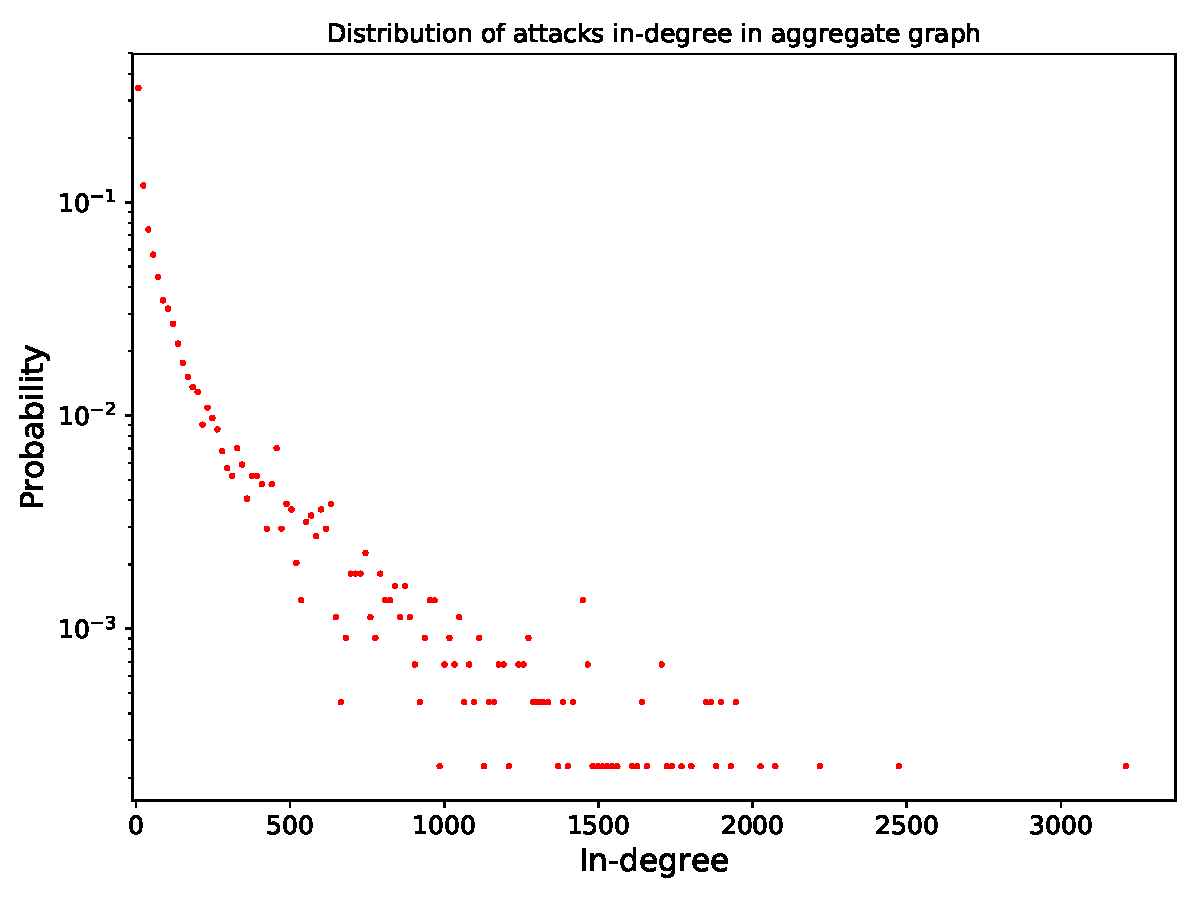
\includegraphics[width = 1.5in]{images/Aggregate/Degree/attacks_in_degree}} &
		\subfloat[Attacks out degree]{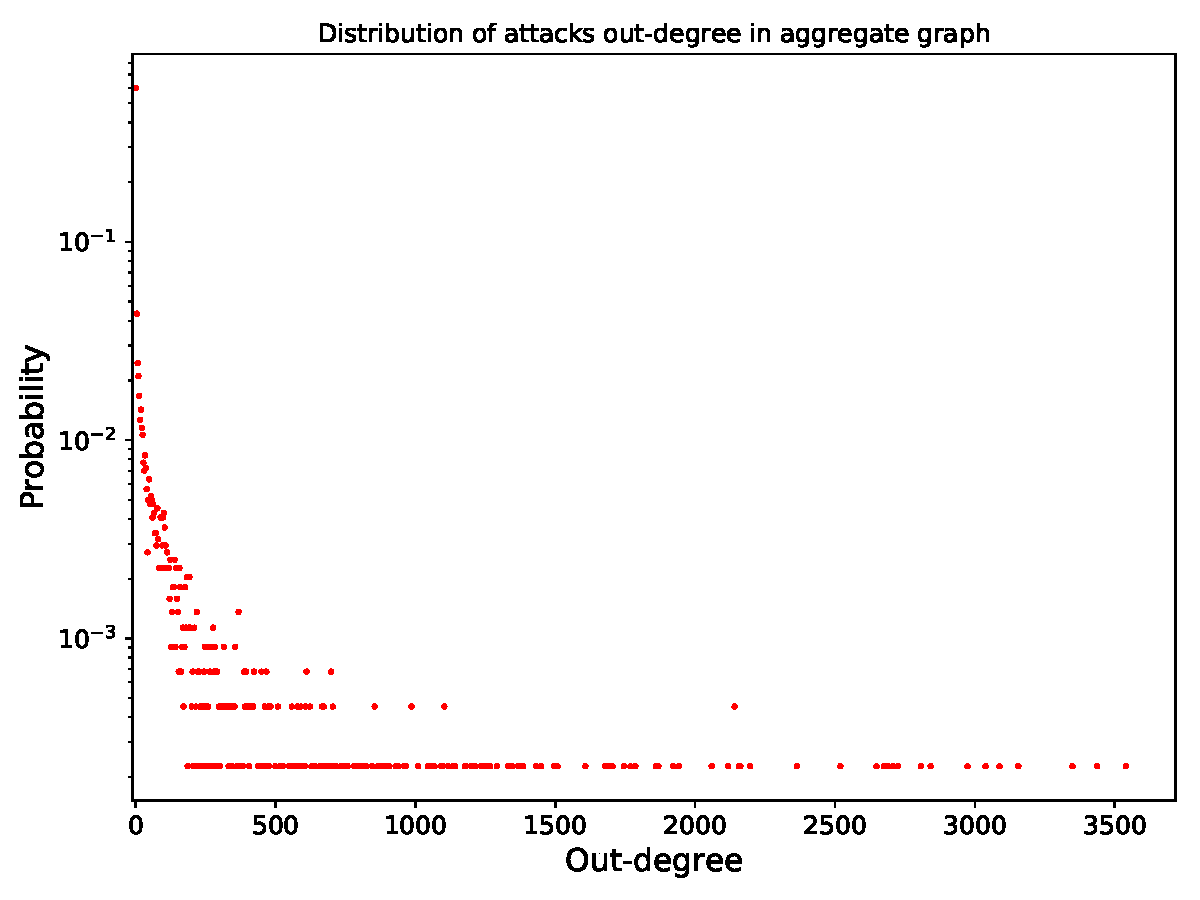
\includegraphics[width = 1.5in]{images/Aggregate/Degree/attacks_out_degree}} &
		\subfloat[Attacks total degree]{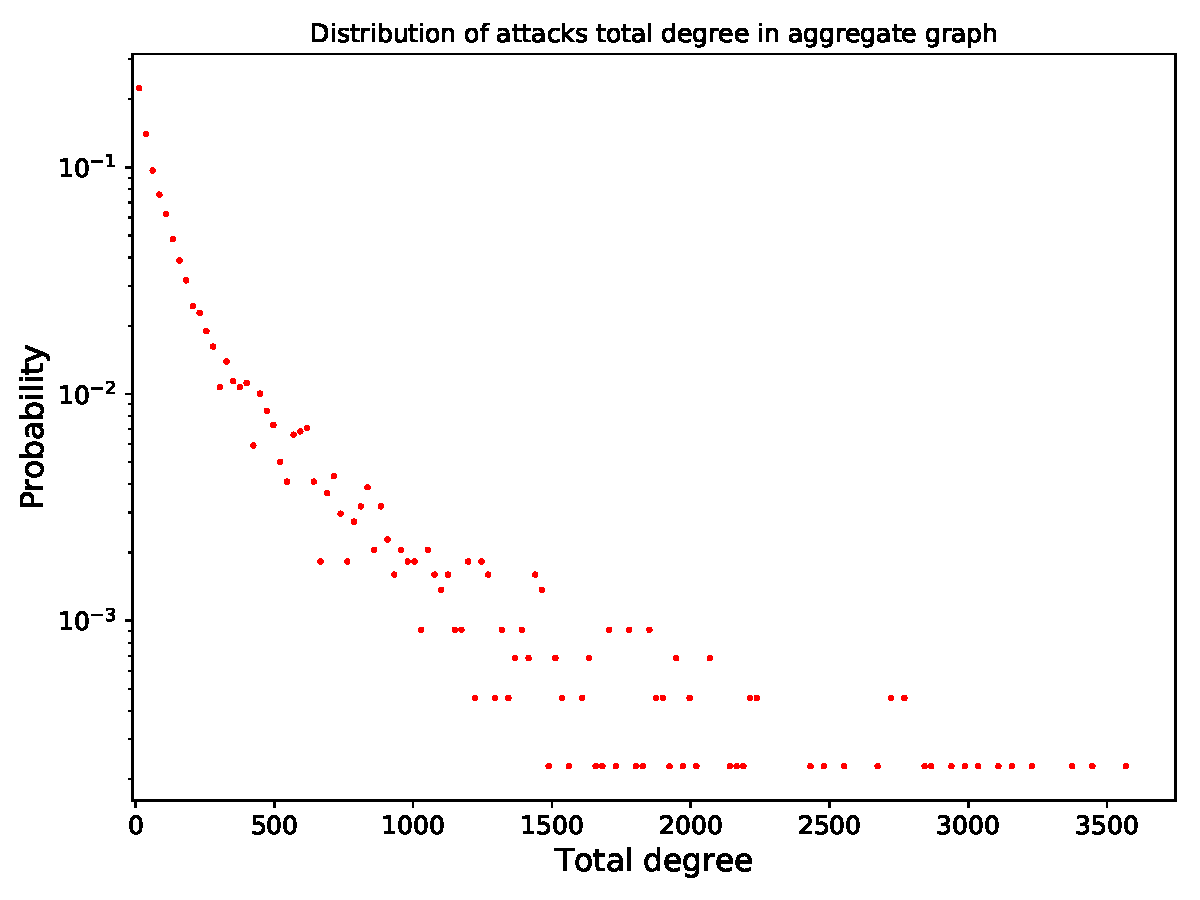
\includegraphics[width = 1.5in]{images/Aggregate/Degree/attacks_total_degree}}\\
		\subfloat[Messages in degree]{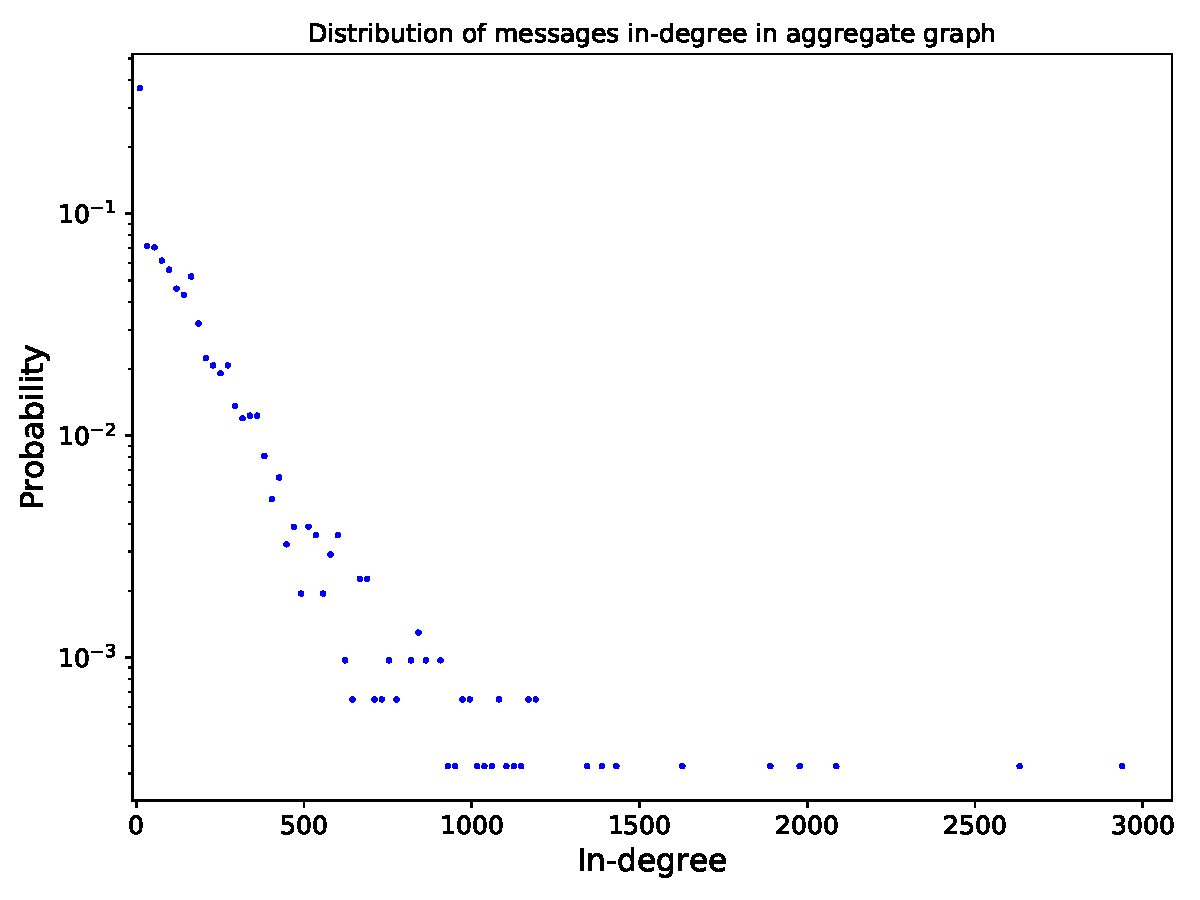
\includegraphics[width = 1.5in]{images/Aggregate/Degree/messages_in_degree}} &
		\subfloat[Messages out degree]{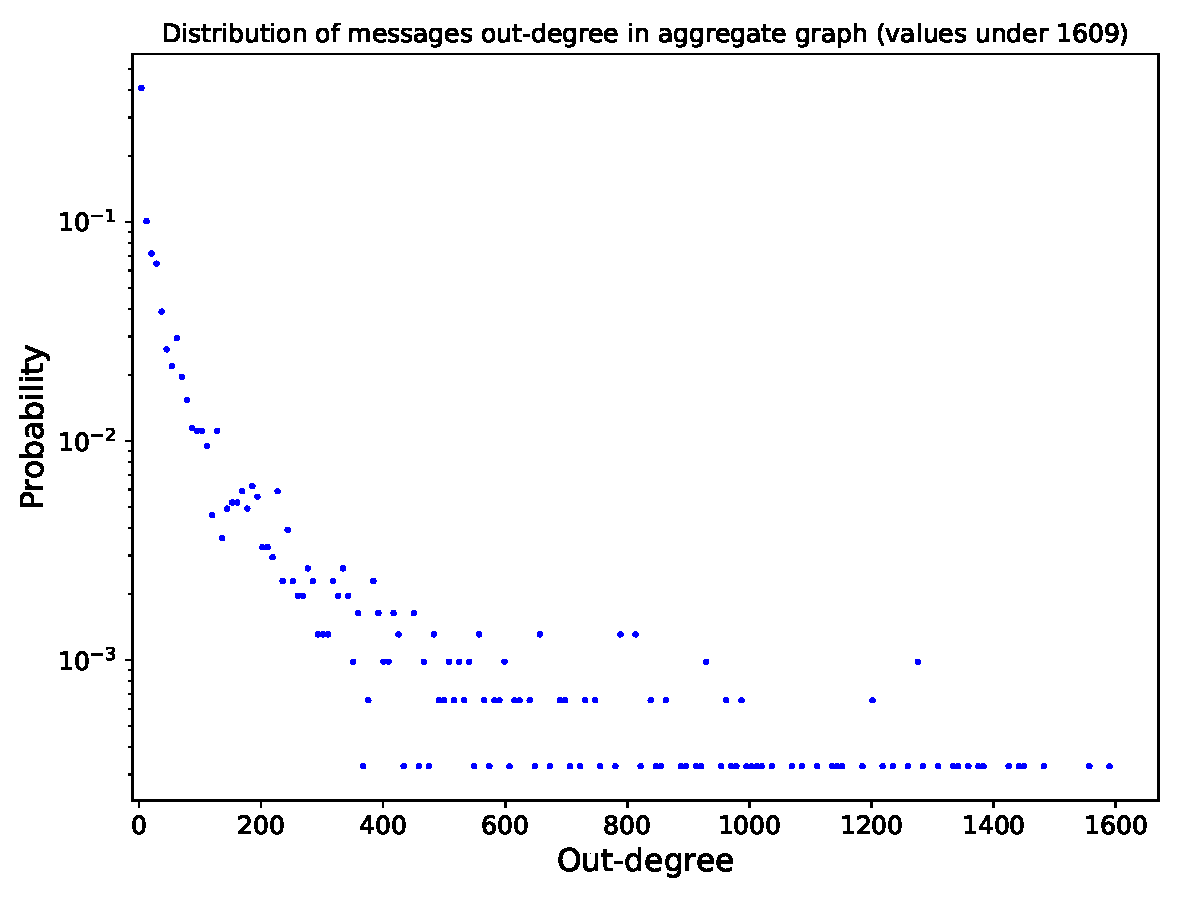
\includegraphics[width = 1.5in]{images/Aggregate/Degree/messages_out_degree}} &
		\subfloat[Messages total degree]{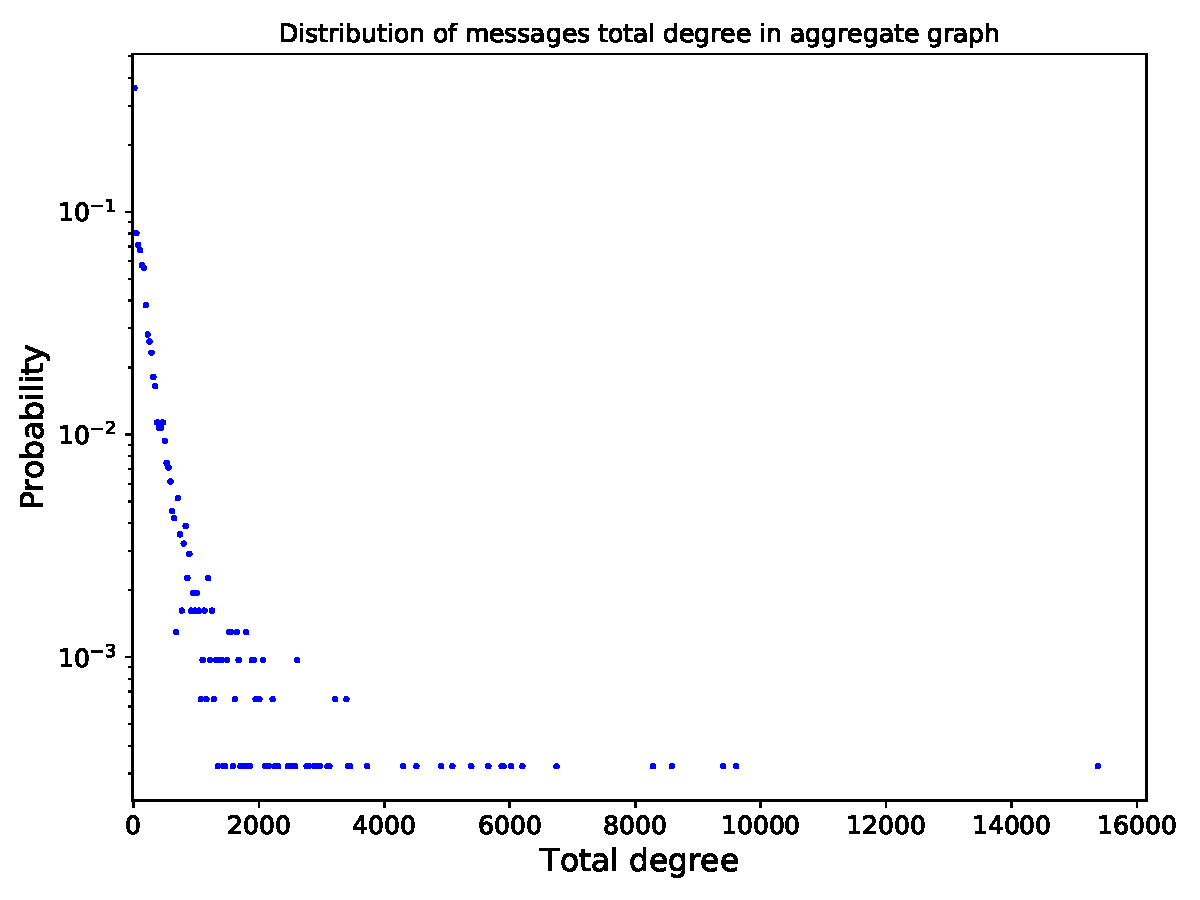
\includegraphics[width = 1.5in]{images/Aggregate/Degree/messages_total_degree}}\\
		\subfloat[Trades in degree]{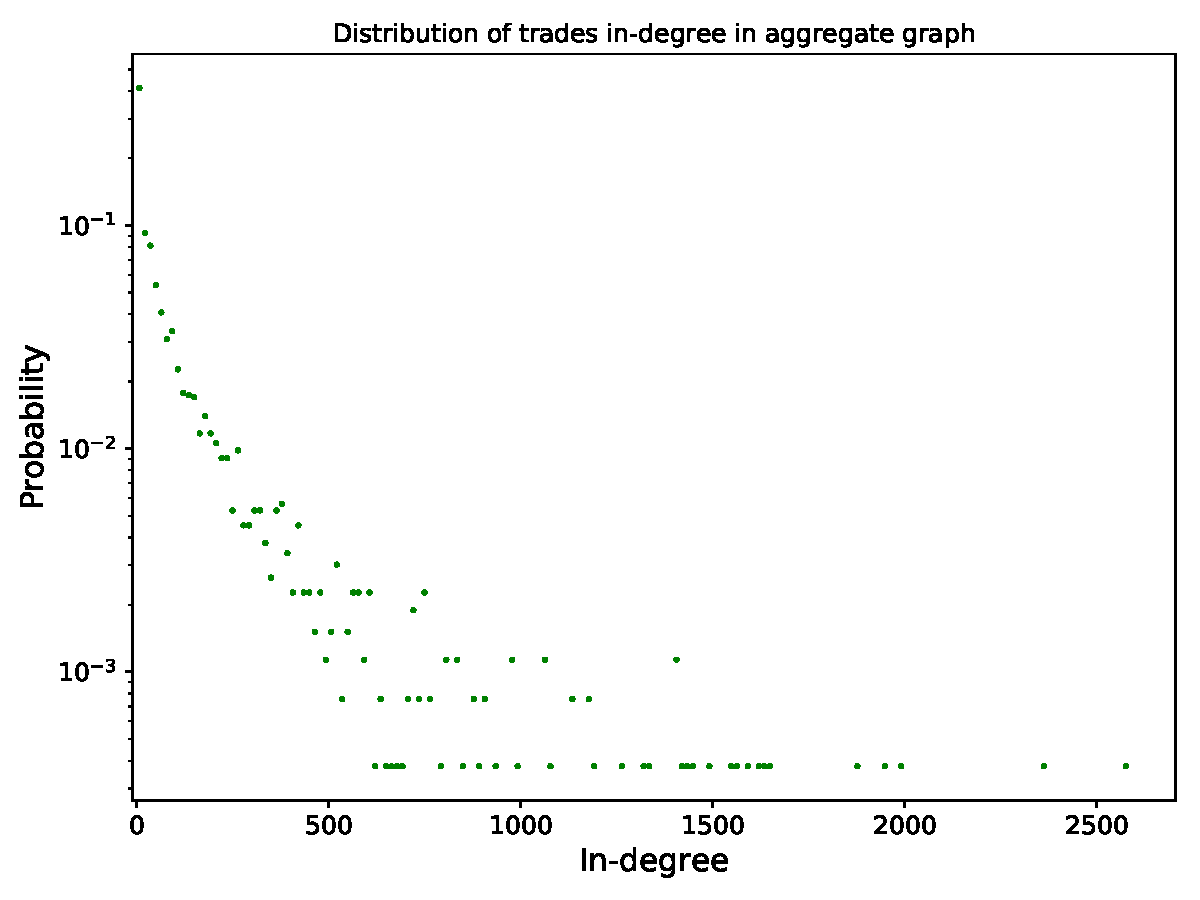
\includegraphics[width = 1.5in]{images/Aggregate/Degree/trades_in_degree}} &
		\subfloat[Trades out degree]{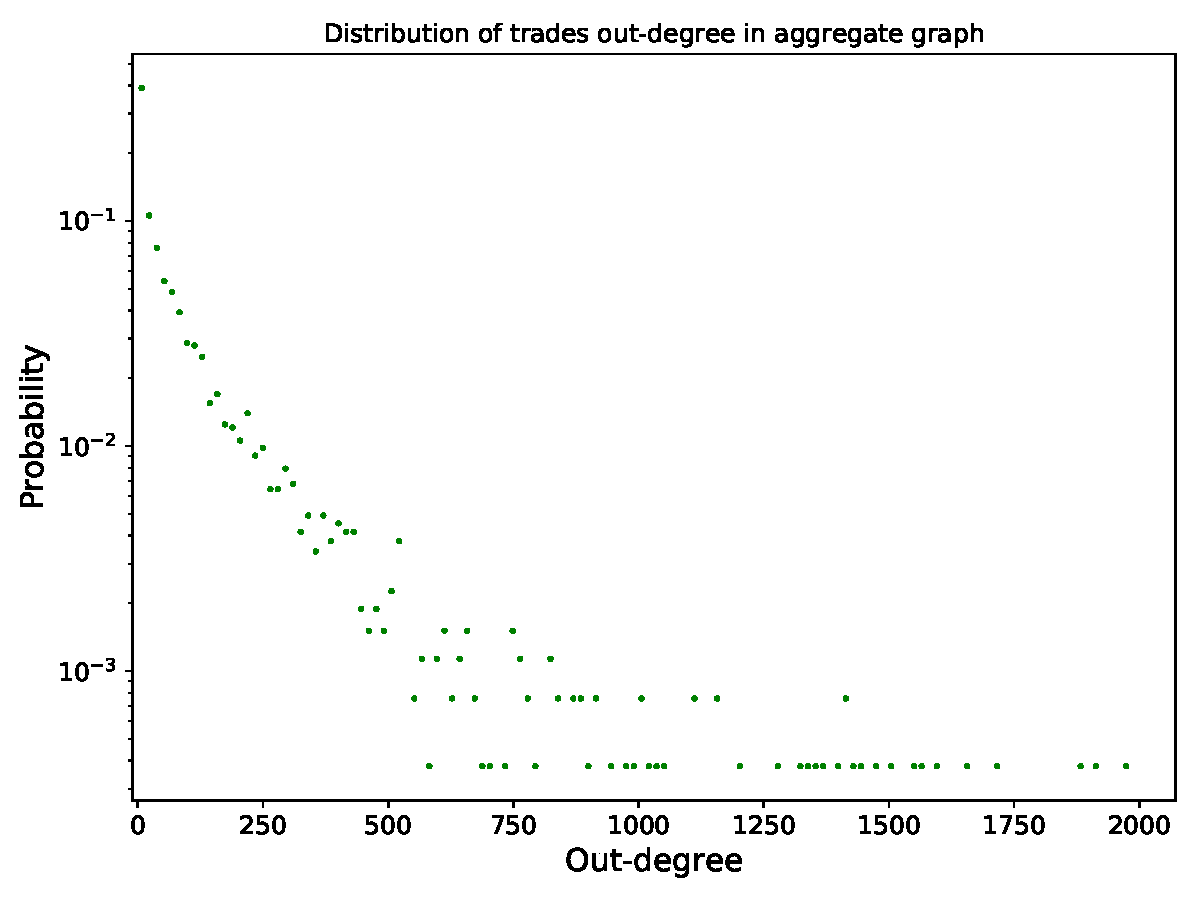
\includegraphics[width = 1.5in]{images/Aggregate/Degree/trades_out_degree}} &
		\subfloat[Trades total degree]{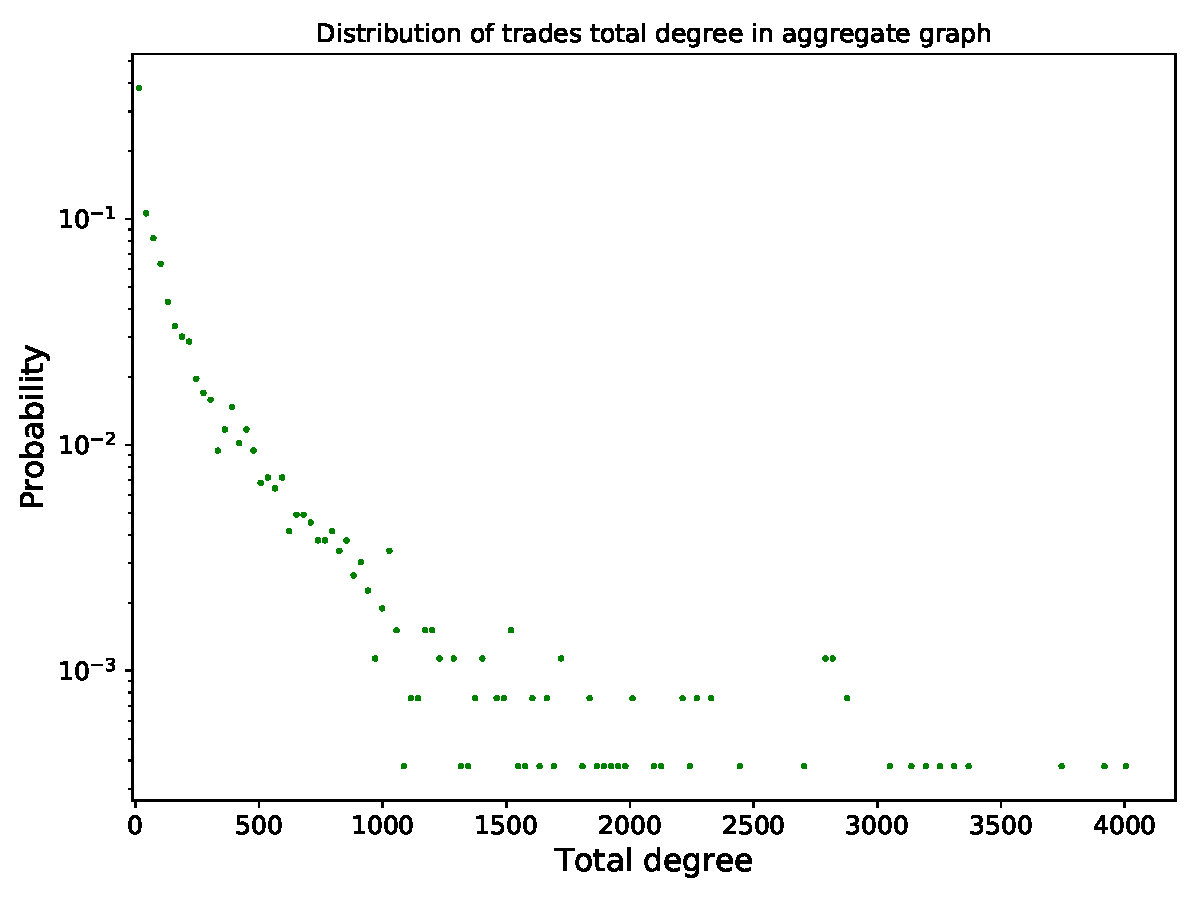
\includegraphics[width = 1.5in]{images/Aggregate/Degree/trades_total_degree}}
	\end{tabular}
	\caption{In-degree, out-degree e grado complessivo dei vari layer della rete.}
	\label{fig:degree}
\end{figure}
 
Sono stati inoltre realizzati dei \textit{jointplot}, per mettere in relazione grado in ingresso ed in uscita dei nodi sui differenti layer, e i risultati sono riportati in Figura \ref{fig:join_degree}. Dai grafici emerge come, per quanto concerne le aggressioni, un elevato numero di attacchi compiuti corrisponde ad un basso numero di attacchi subiti, e viceversa.\\
Per gli scambi la situazione è diametralmente opposta, con un grafico che si distribuisce principalmente sulla diagonale, dove il numero di trade in uscita è pari a quello in entrata.\\
Il grafico dei messaggi risulta essere più variegato, con tendenze a ricevere più messaggi di quelli inviati, ma non emerge un chiaro comportamento come nei due casi precedenti
\begin{figure}
	\subfloat[Jointplot attacchi.]{%
		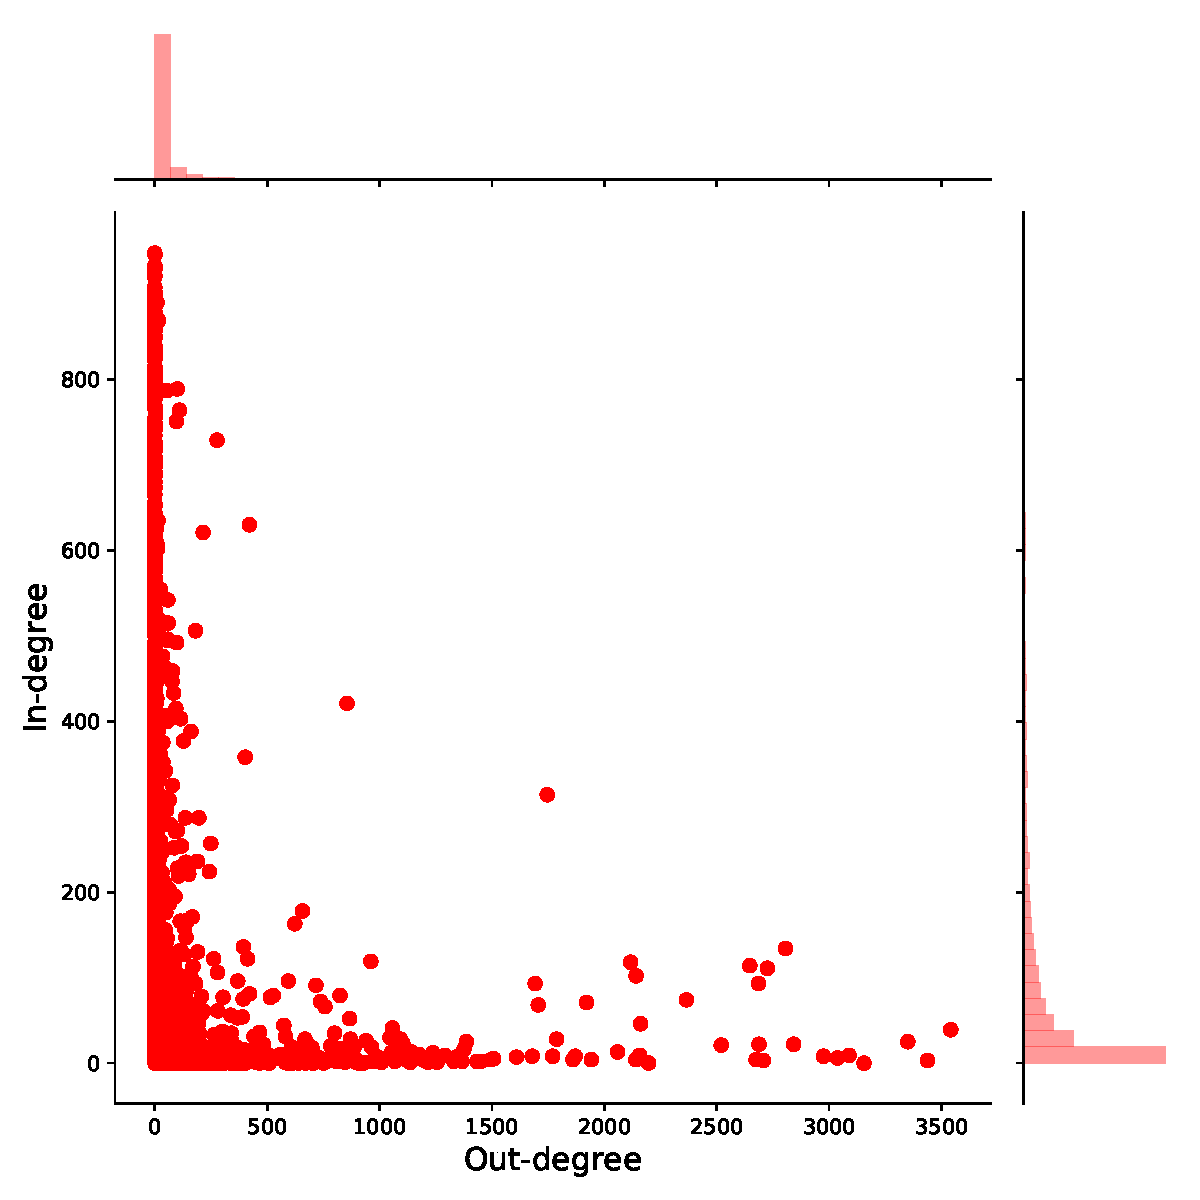
\includegraphics[width=.55\linewidth]{images/Aggregate/Degree/jointplot/attacks_jointplot_no_outliers}
	}
	\hfill
	\subfloat[Jointplot messaggi.]{%
	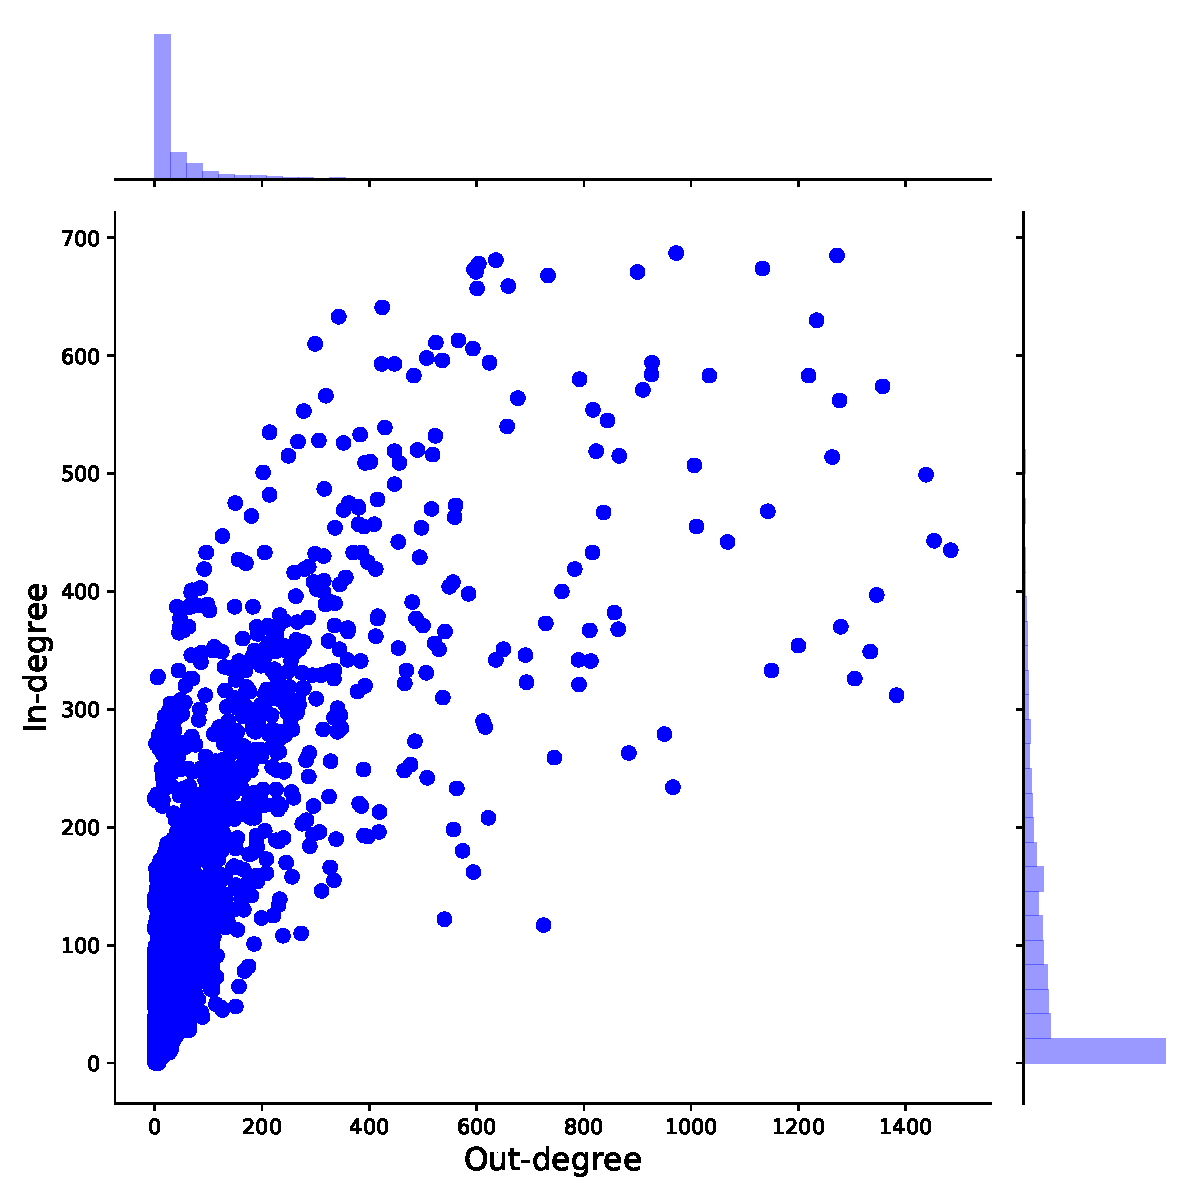
\includegraphics[width=.55\linewidth]{images/Aggregate/Degree/jointplot/messages_jointplot_no_outliers}
	}
	\hfill
	\subfloat[Jointplot trade.]{%
	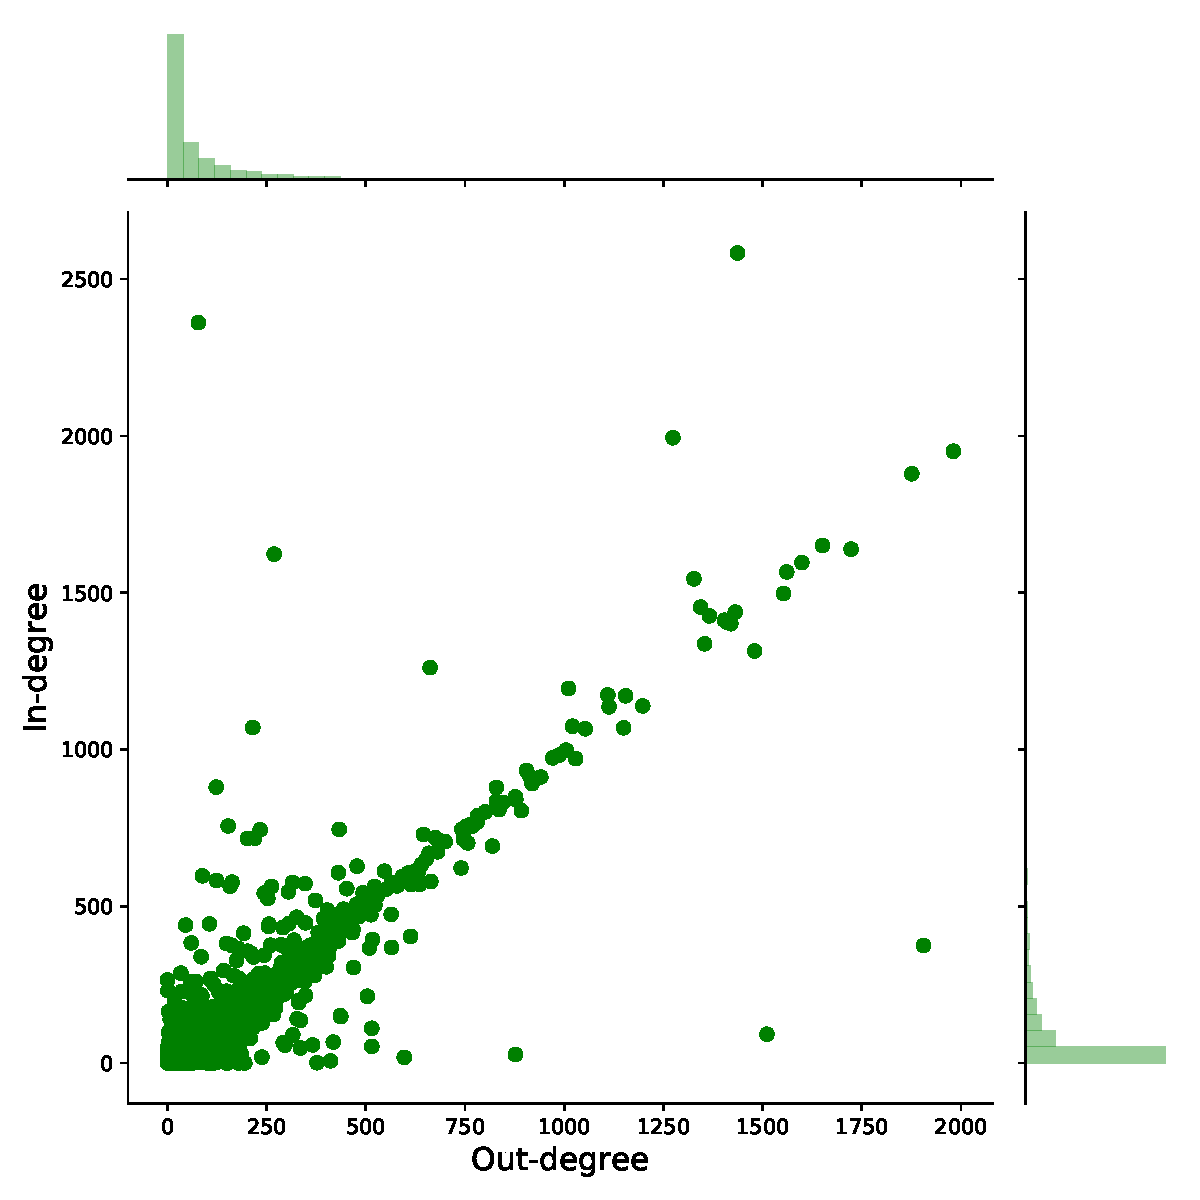
\includegraphics[width=.55\linewidth]{images/Aggregate/Degree/jointplot/trades_jointplot}
	}
	\caption{Jointplot che pongono in relazione in-degree e out-degree del layer specificato.}
	\label{fig:join_degree}
\end{figure}

In ultimo, sono stati generati i \textit{jointplot} che pongono in relazione gli out-degree di messaggi e attacchi o trade, rispettivamente in Figura \ref{subfig:joint_m_a} e \ref{subfig:joint_m_t}. Dal primo grafico si evince come numero di attacchi e numero di messaggi siano solitamente inversamente proporzionali, mentre non vi sembra essere una stretta relazione tra messaggi e scambi commerciali.
\begin{figure}
	\subfloat[Jointplot tra messaggi e attacchi.\label{subfig:joint_m_a}]{%
		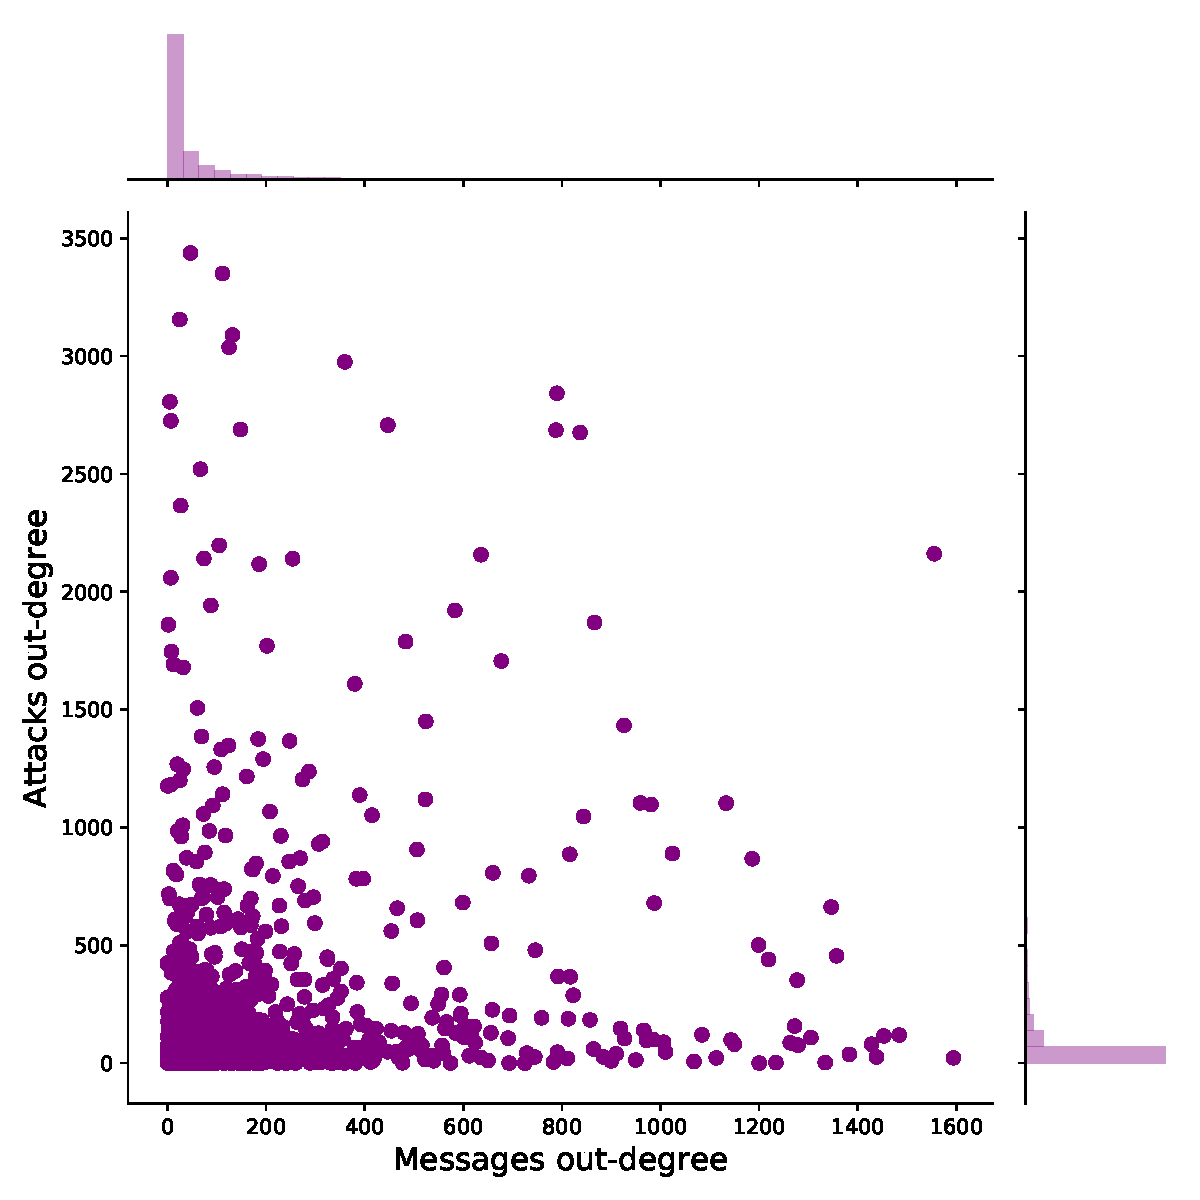
\includegraphics[width=.55\linewidth]{images/Aggregate/Degree/jointplot/messages_out-degree_vs_attacks_out-degree}
	}
	\hfill
	\subfloat[Jointplot tra messaggi e scambi.\label{subfig:joint_m_t}]{%
		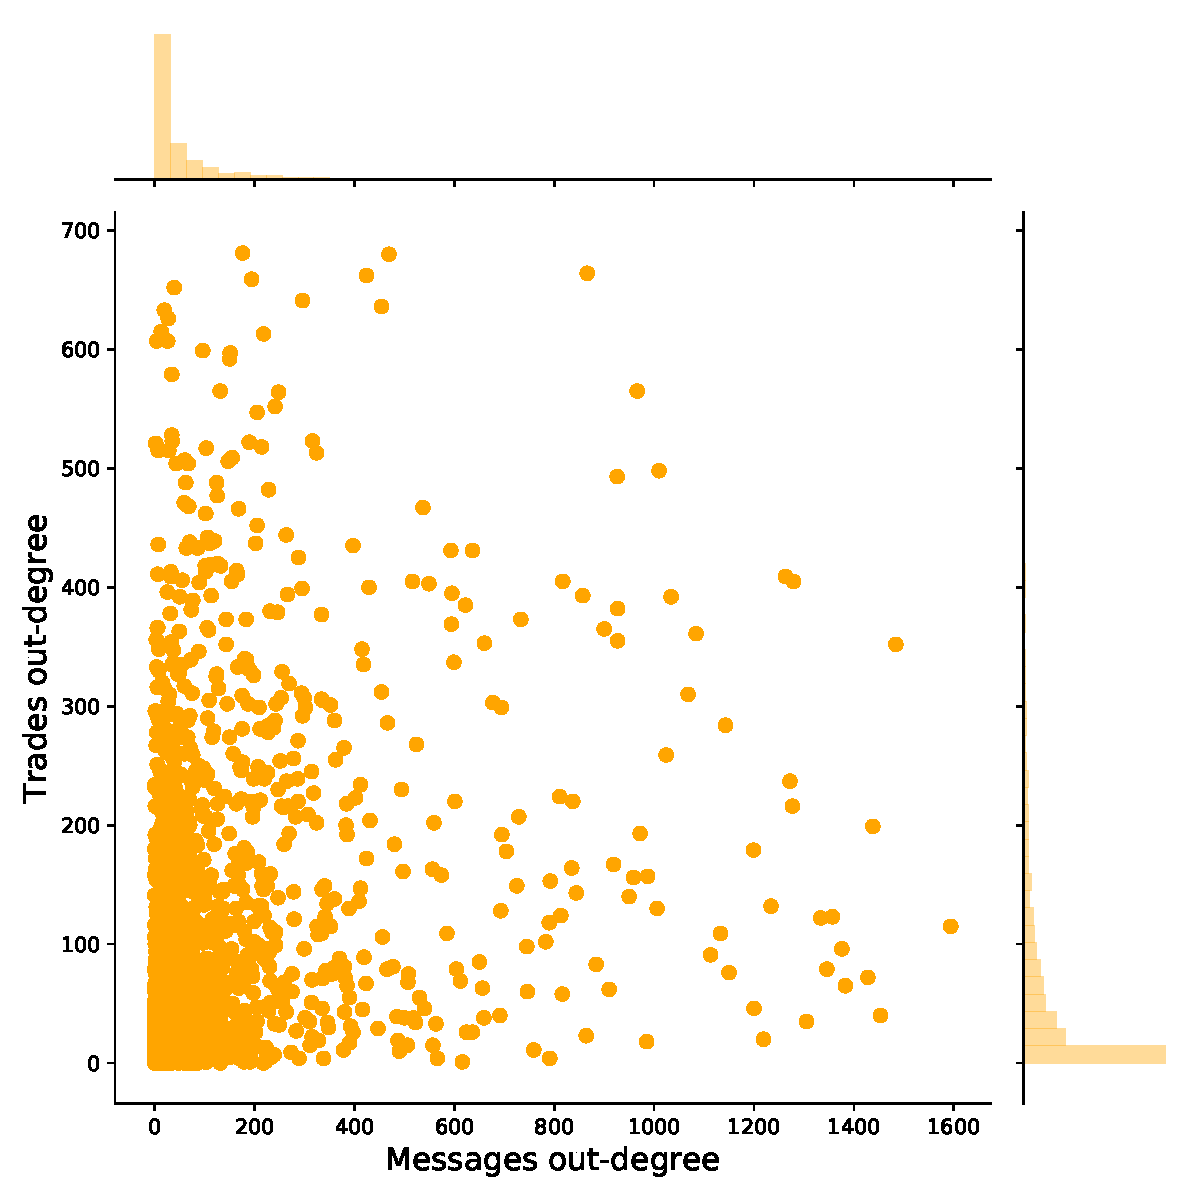
\includegraphics[width=.55\linewidth]{images/Aggregate/Degree/jointplot/messages_out-degree_vs_trades_out-degree}
	}
	\caption{Jointplot che pongono in relazione out-degree dei diversi layer.}
	\label{fig:join_mixed}
\end{figure}

\subsection{Misure di centralità}
\label{subsec:centrality}
Per quanto riguarda le misure di centralità, abbiamo deciso di concentrare i nostri approfondimenti esclusivamente sui layer di messaggi e scambi, in quanto sulla rete di attacchi il calcolo di queste misure risulta essere poco sensato (non vi è alcun flusso informativo).\\
Le misure analizzate per i due layer considerati sono:
\begin{itemize}
	\item Betweenness: misura che rappresenta il grado di informazione passante per un dato nodo. Un elevato valore indica un nodo centrale nel flusso informativo / commerciale, con una grande capacità di collegamento tra porzioni della rete.
	\item PageRank: calcola l'importanza di un nodo grazie al numero di archi entranti e al peso dei nodi che lo referenziano. Fornisce un'informazione pesata e più specifica rispetto al semplice grado in ingresso.
\end{itemize}

Per il layer dei messaggi, i grafici delle due misure analizzate, riportati in Figura \ref{fig:messages_centrality}, mostrano una predominanza del contatto diretto rispetto al passaggio di informazione secondo una scala di gradi. Un distribuzione dei valori di betweenness concentrata in valori molto bassi, indica la presenza di molti collegamenti alternativi tra due nodi: non si presenta quindi la situazione di un passaggio "forzato" per un determinato nodo. PageRank mostra un andamento simile, non individuando chiaramente dei nodi predominanti sugli altri. Si noti che dal dataset sono stati rimossi tutti i messaggi di \textit{broadcast}, ovvero le comunicazioni inviate dai gestori delle alleanze a tutti i membri di essa: questo ha certamente influenzato una compressione di valori delle due misure precedentemente analizzate.\\ 
\begin{figure}
	\subfloat[Centralità Betweenness.]{%
		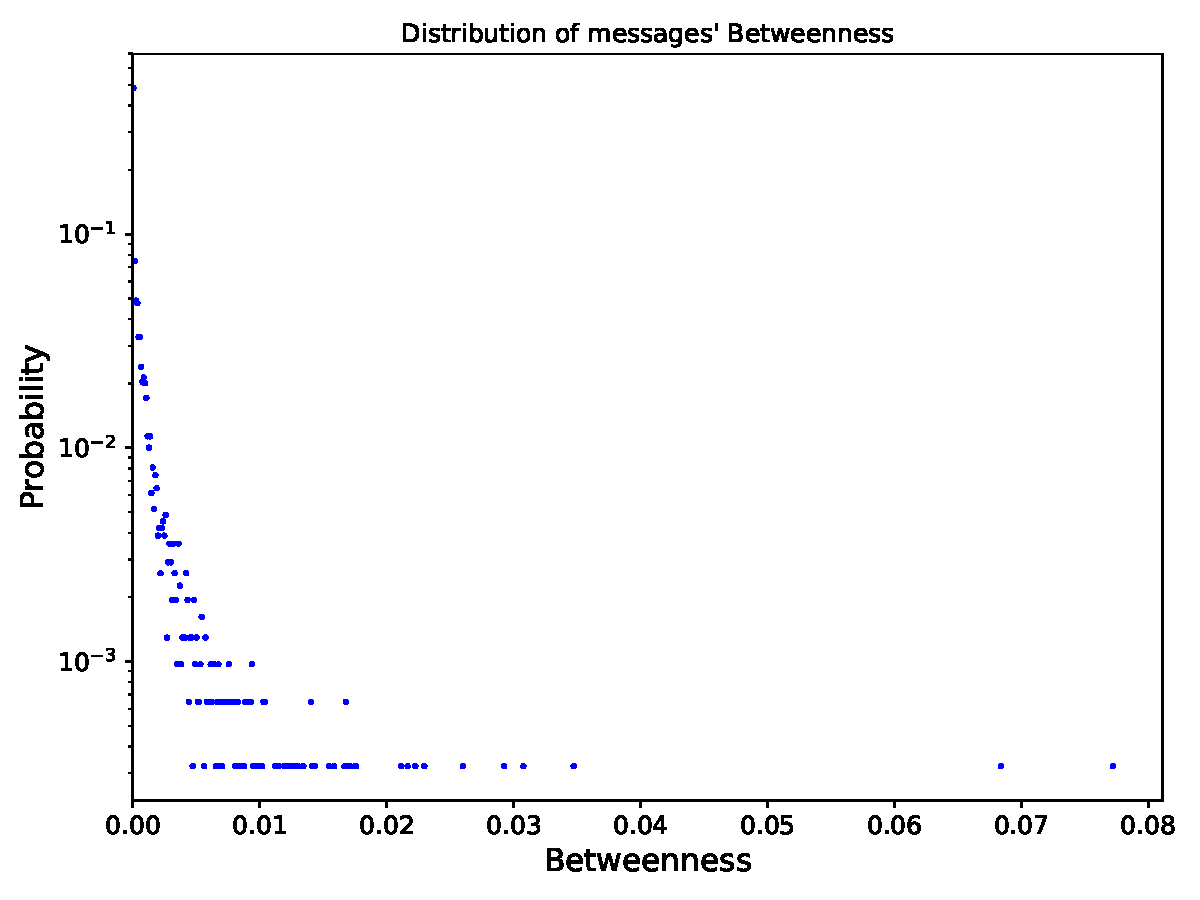
\includegraphics[width=.55\linewidth]{images/Aggregate/Centrality/messages_betweenness}
	}
	\hfill
	\subfloat[Centralità Pagerank.]{%
		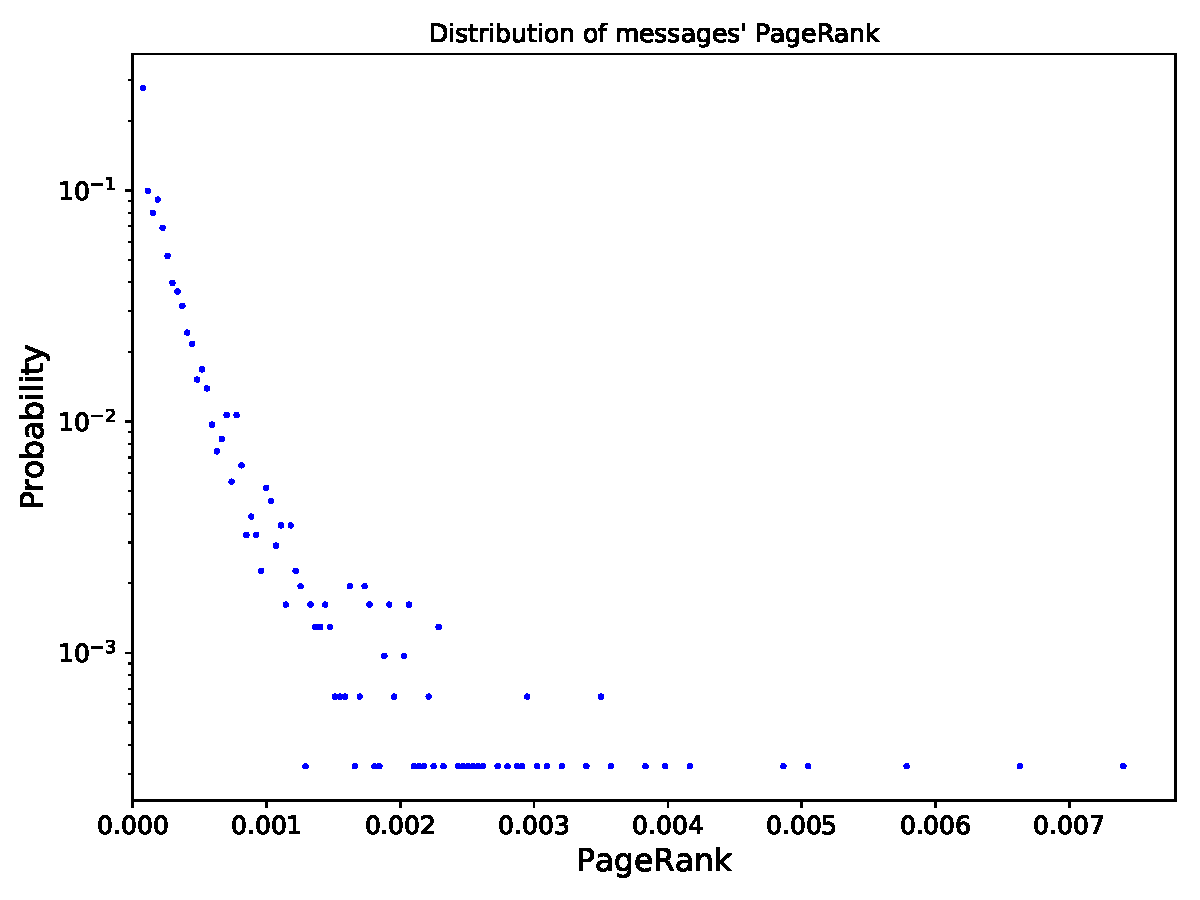
\includegraphics[width=.55\linewidth]{images/Aggregate/Centrality/messages_PageRank}
	}
	\caption{Grafici delle misure di centralità calcolate sul layer dei messaggi.}
	\label{fig:messages_centrality}
\end{figure}
Lo stesso comportamento è mostrato dall'analisi del grafo degli scambi (in Figura \ref{fig:trades_centrality}), con valori della betweenness ancora più compressi rispetto ai messaggi. Ciò è probabilmente dovuto all'assenza di figure di passaggio delle merci: non vi è un "mercante" che acquista beni da un insieme di villaggi per poi rivendere ad altri, ma i giocatori sono liberi di commerciare direttamente tra loro.
\begin{figure}
	\subfloat[Centralità Betweenness.]{%
		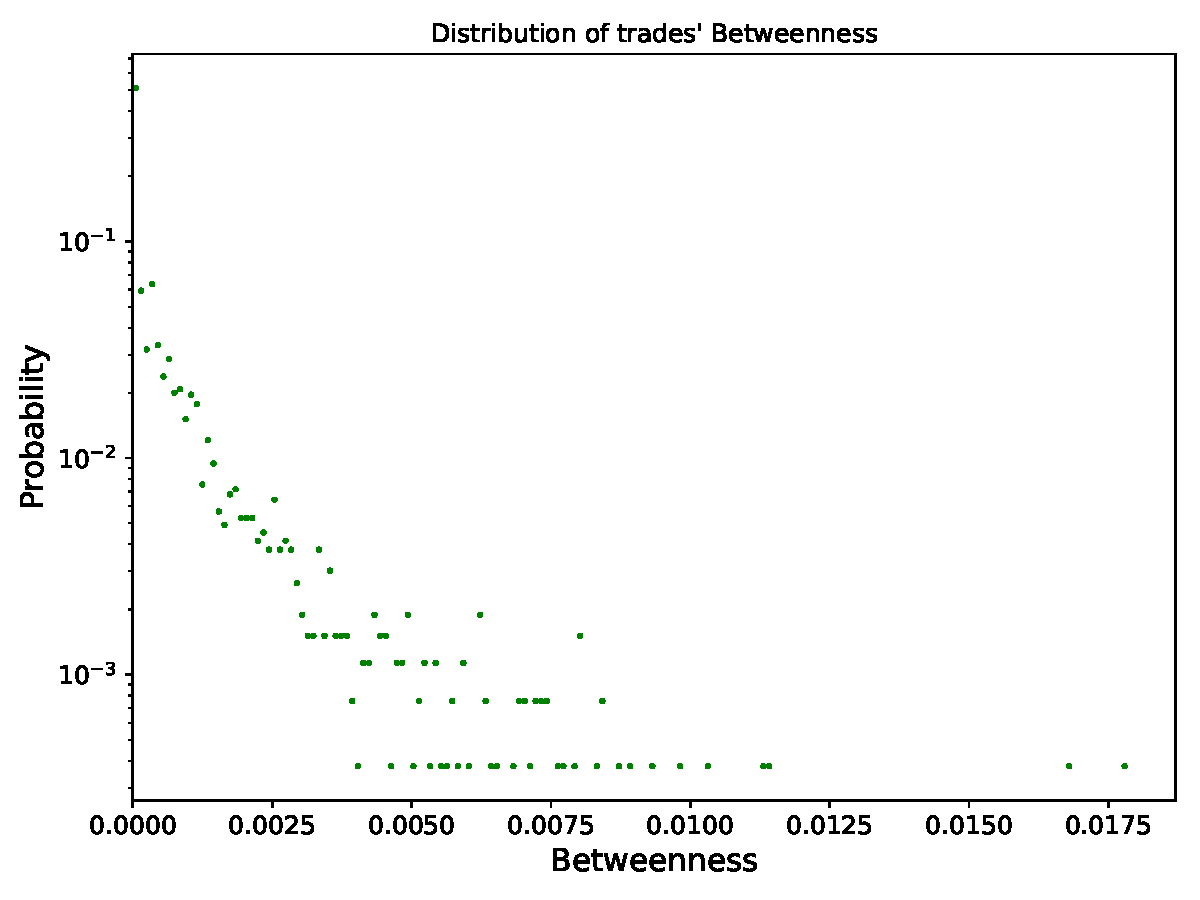
\includegraphics[width=.55\linewidth]{images/Aggregate/Centrality/trades_betweenness}
	}
	\hfill
	\subfloat[Centralità Pagerank.]{%
		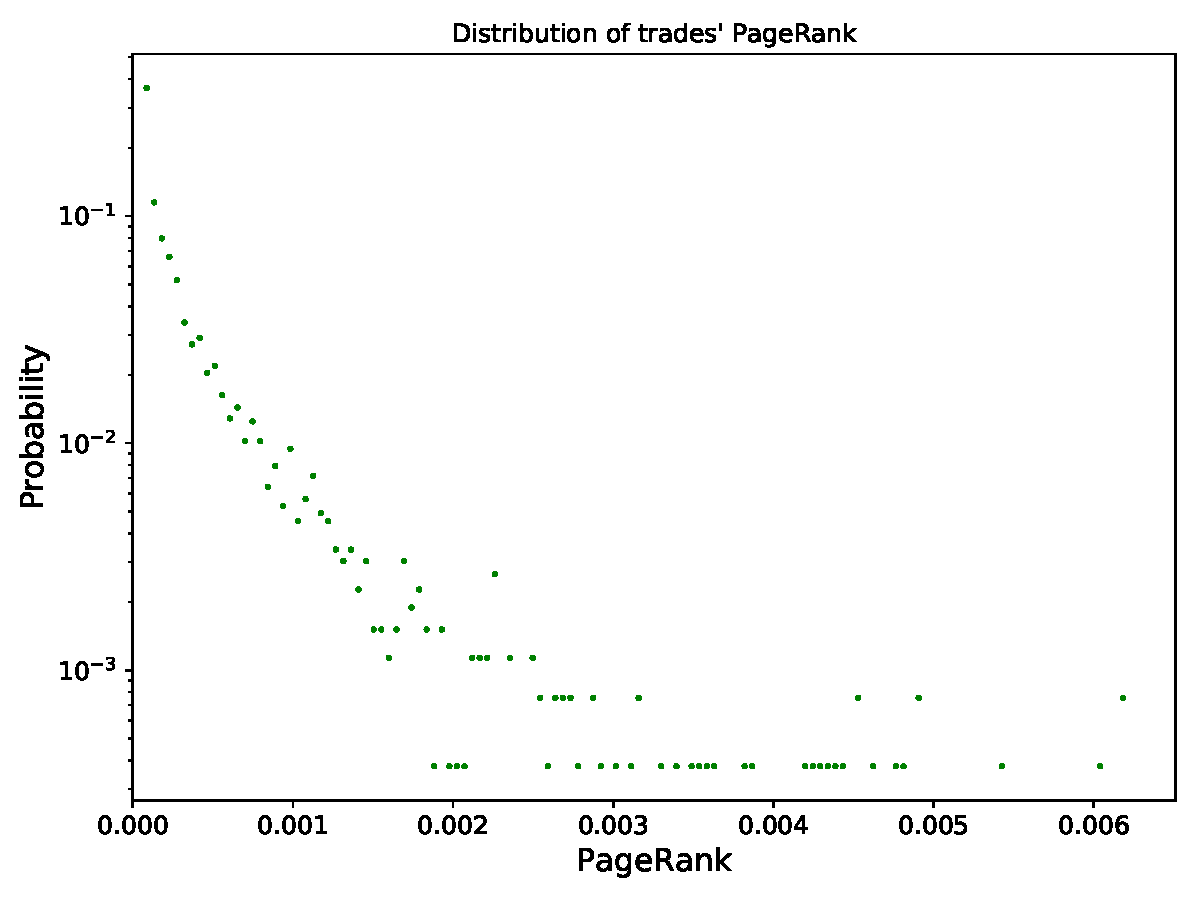
\includegraphics[width=.55\linewidth]{images/Aggregate/Centrality/trades_PageRank}
	}
	\caption{Grafici delle misure di centralità calcolate sul layer dei trade.}
	\label{fig:trades_centrality}
\end{figure}

Abbiamo infine generato i jointplot delle due misure analizzate, per individuare possibili correlazioni tra i valori delle due. I risultati, riportati in Figura \ref{fig:joint_centrality}, mostrano come la maggioranza dei nodi si concentri nei pressi dell'origine degli assi, a cui corrispondono bassi valori di entrambe le misure. Sono apprezzabili diversi outliers in entrambi i grafici, che mostrano \todo{indagare su questi outliers}
\begin{figure}
	\subfloat[Jointplot messaggi.]{%
		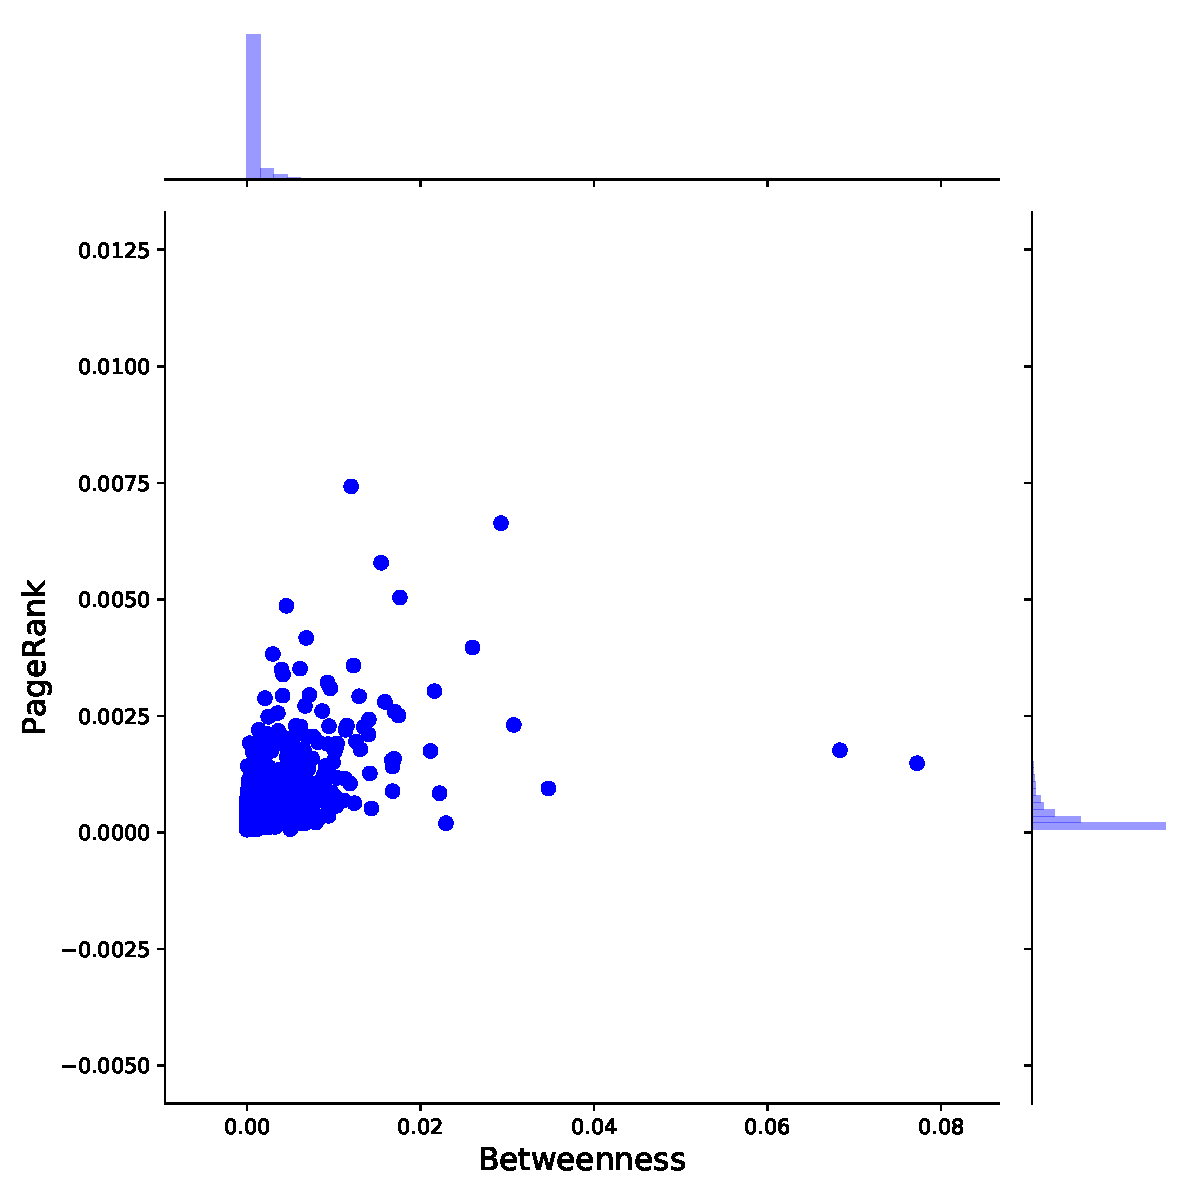
\includegraphics[width=.55\linewidth]{images/Aggregate/Centrality/messages_jointplot}
	}
	\hfill
	\subfloat[Jointplot trade.]{%
		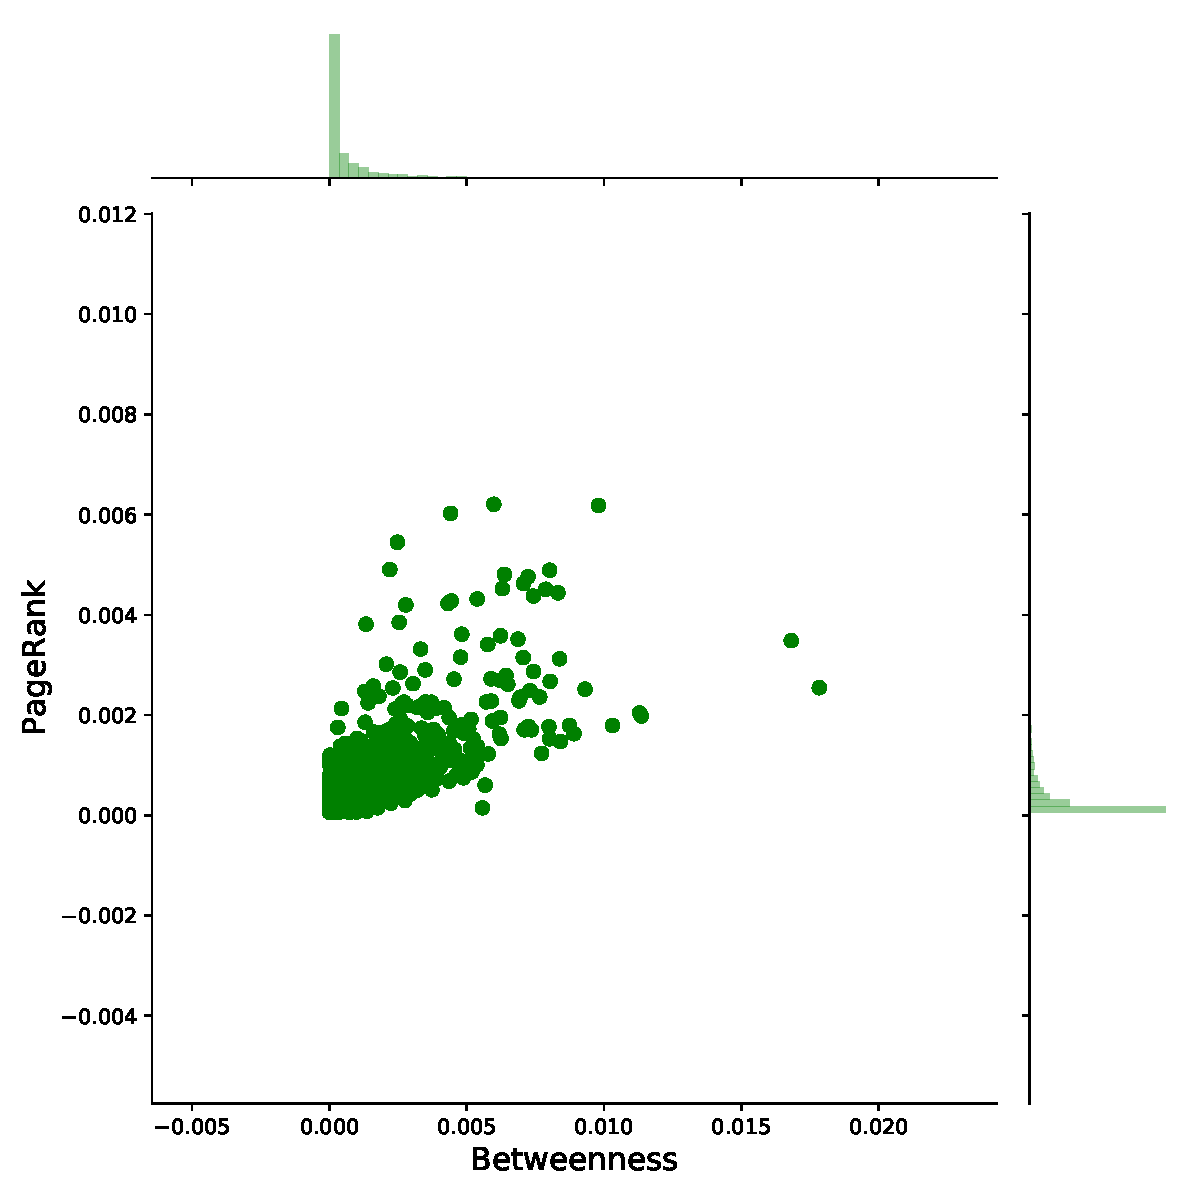
\includegraphics[width=.55\linewidth]{images/Aggregate/Centrality/trades_jointplot}
	}
	\caption{Jointplot delle misure di centralità calcolate rispettivamente sui messaggi e sugli scambi.}
	\label{fig:joint_centrality}
\end{figure}


\subsection{Coefficiente di clustering medio}
Un'ulteriore misura analizzata è stata il coefficiente medio di clustering, ovvero la misura della tendenza di un nodo a formare un cricca (i.e. grafo completo). Questo comportamento è solito rilevarsi nelle reti sociali, dove i nodi tendono a formare delle community dense e coese rispetto al resto del grafo. Essendo questa una misura media, bisogna considerare il fatto che la maggior parte dei nodi non facciano parte di alcuna community, e questo influenzi molto il valore medio ottenuto: useremo i risultati di questa analisi come metro di paragone per i successivi studi sulle alleanze. 
I risultati ottenuti sono riportati in Figura \ref{fig:clustering}: vediamo come nel layer dei messaggi, che possiamo considerare una rete sociale, i valori medi sono decisamente maggiori rispetto alla rete degli scambi, dove i vicini di un nodo non necessariamente sono soliti commerciare tra loro. Ci possiamo altresì aspettare che i nodi del vicinato di x siano più propensi a conoscersi e a comunicare tra loro.
\ref{fig:messages_centrality}, mostrano 
\begin{figure}
	\subfloat[Coefficiente di clustering medio per i messaggi.]{%
		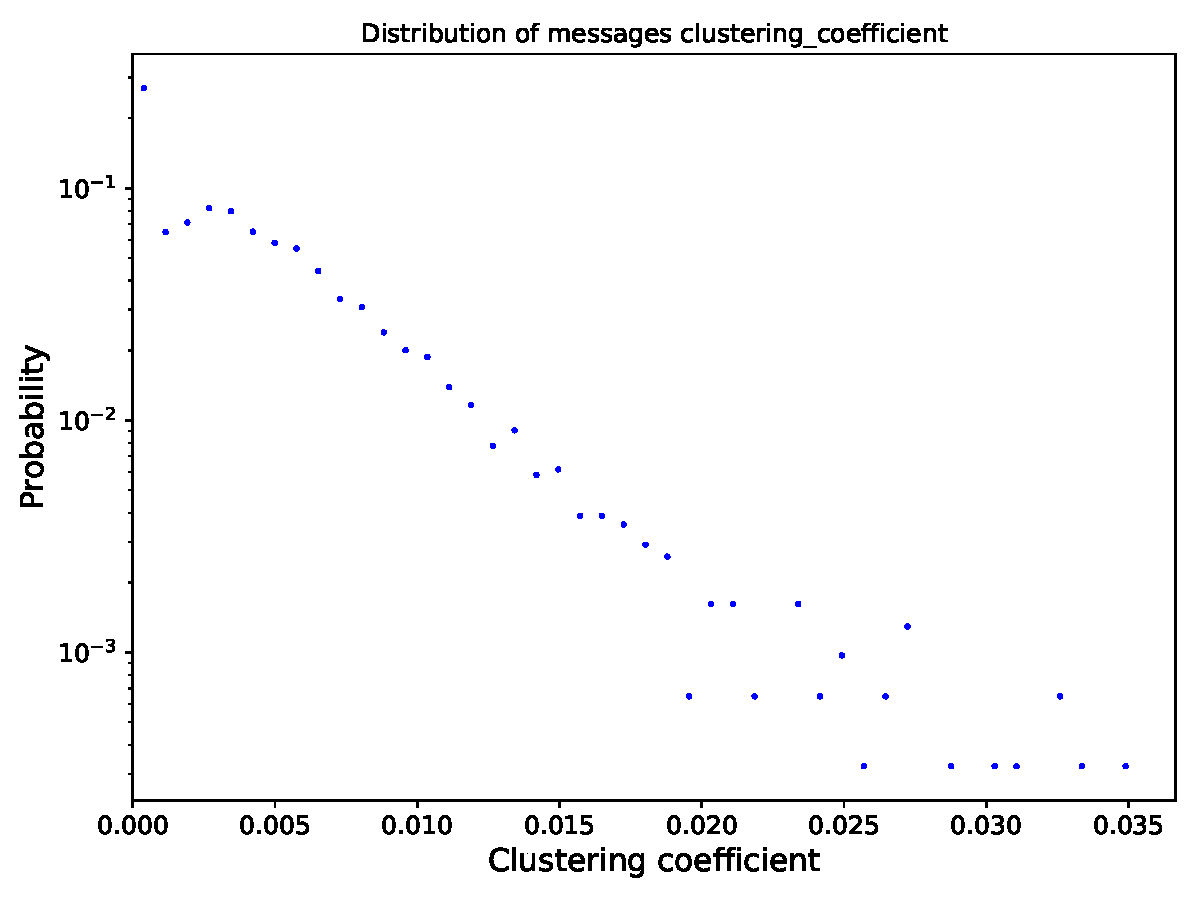
\includegraphics[width=.55\linewidth]{images/Aggregate/Clustering/messages}
	}
	\hfill
	\subfloat[Coefficiente di clustering medio per i trade.]{%
		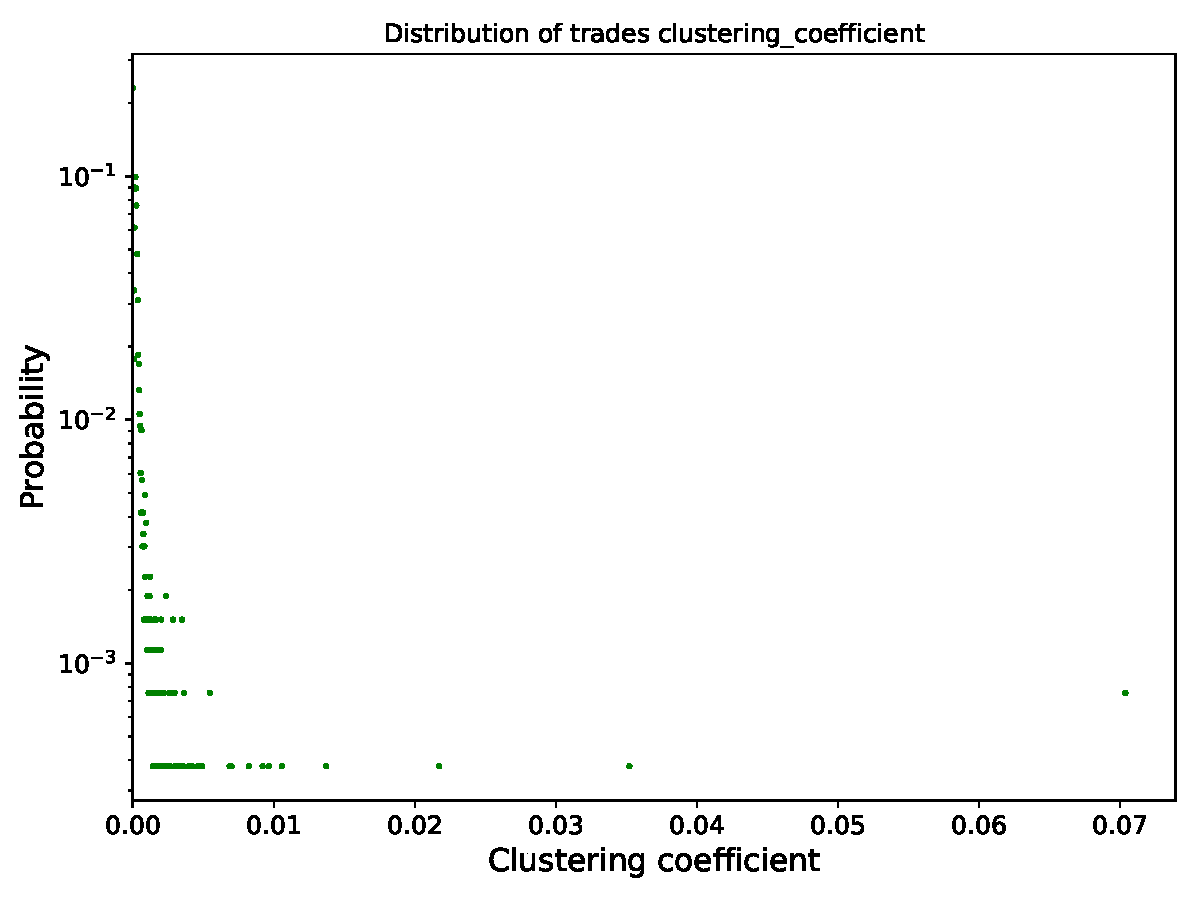
\includegraphics[width=.55\linewidth]{images/Aggregate/Clustering/trades}
	}
	\caption{Grafici delle misure di centralità calcolate sul layer dei messaggi.}
	\label{fig:clustering}
\end{figure}

\newpage 
\section{Analisi delle attività}
Un'ulteriore analisi condotta sul dataset è stata la distribuzione giornaliera di attività durante il periodo analizzato: ci siamo chiesti se fosse possibile delineare una qualche relazione tra i dati disponibili, in particolare tra numero di giocatori ed attività.\\
Il numero di giocatori attivi sul server in almeno uno dei tre layer è rappresentato in Figura \ref{fig:playereachday}, dove si può notare un drastico calo al giorno 5.
\begin{figure}
	\centering
	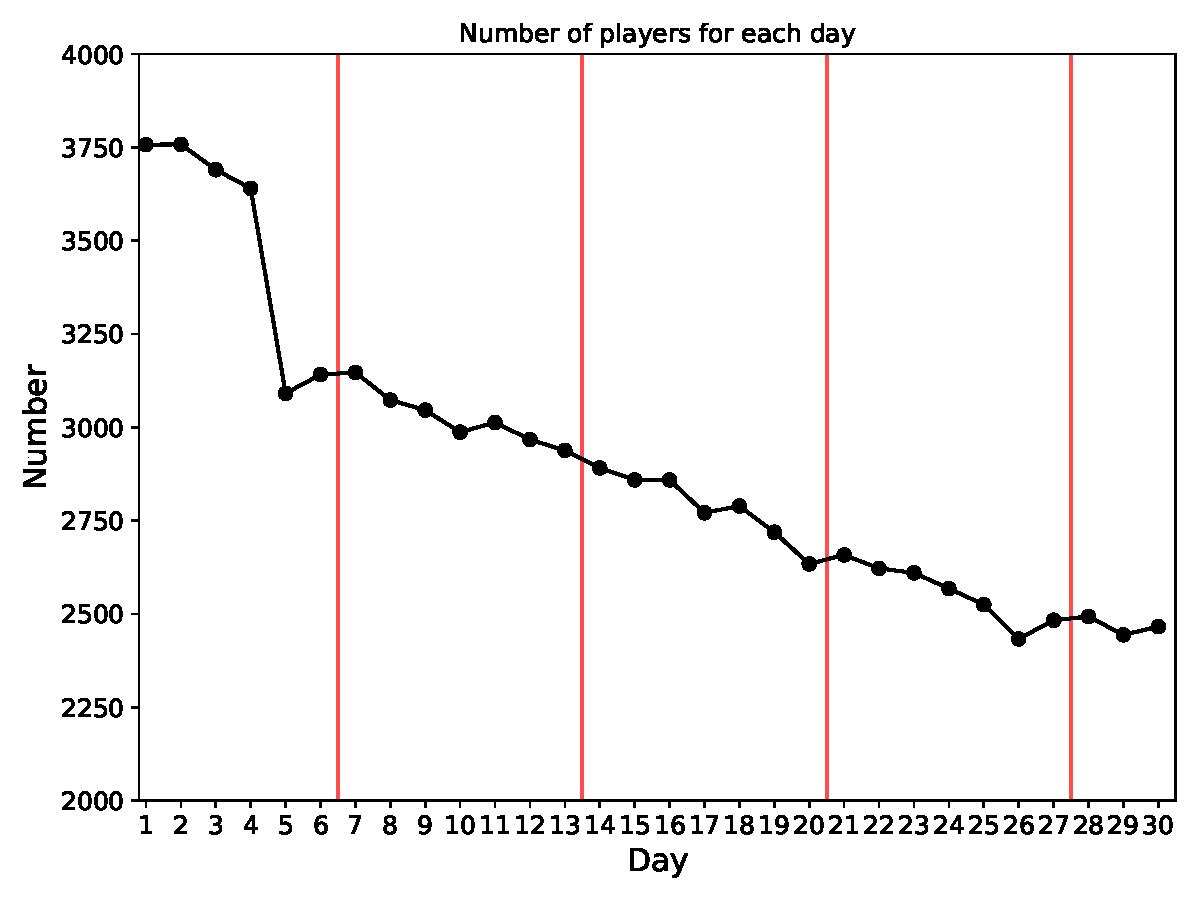
\includegraphics[width=0.8\linewidth]{images/Activity/player_each_day}
	\caption{Numero di giocatori attivi in un dato giorno. rappresentano l'inizio di una nuova settimana.}
	\label{fig:playereachday}
\end{figure}
Come mostrato in Figura \ref{fig:activity_each_day}, complessivamente il numero di azioni eseguite dai giocatori decresce lungo il periodo analizzato, con picchi durante i week-end e le festività. 
\begin{figure}
	\subfloat[Numero di archi presenti nei vari layer ad un dato giorno.]{%
		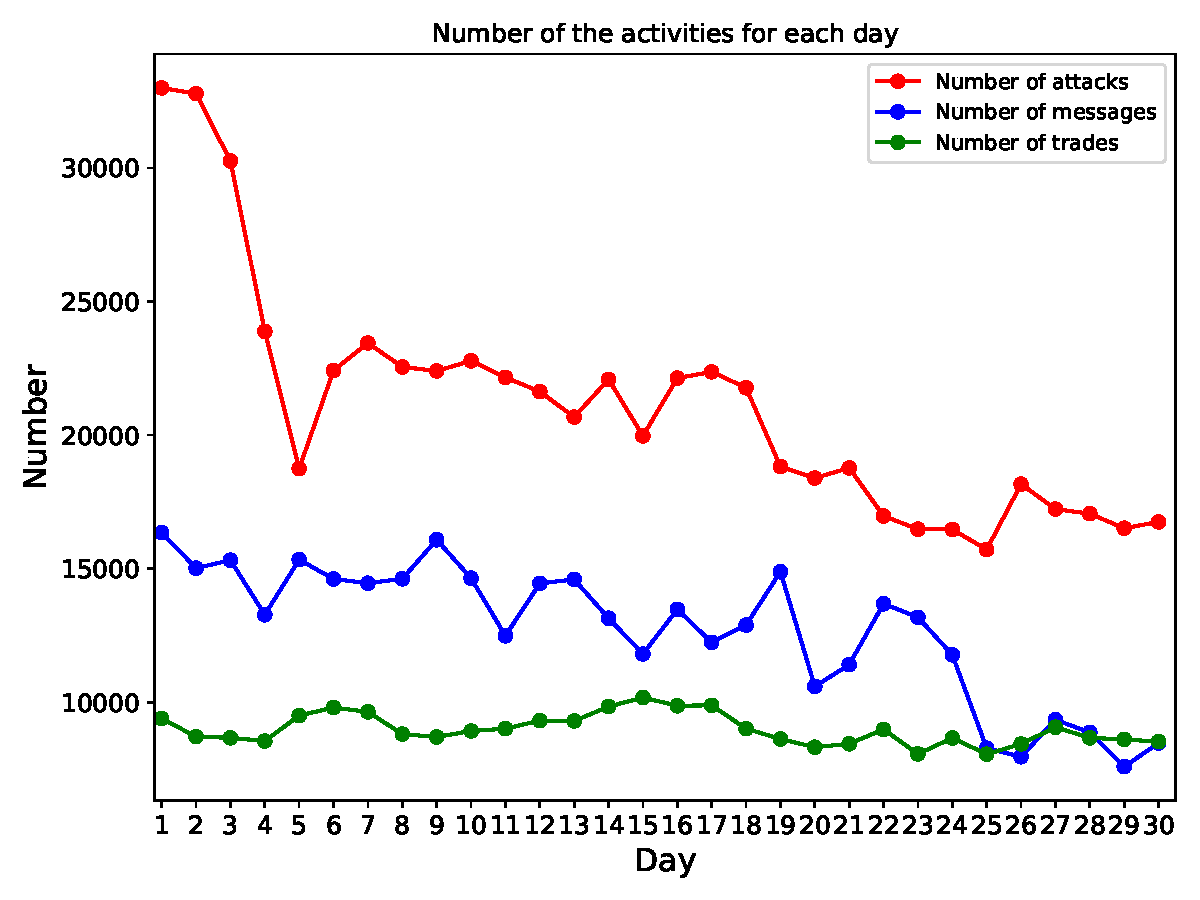
\includegraphics[width=.45\linewidth]{images/Activity/n_each_activity_each_day}
	}
	\hfill
	\subfloat[Somma del numero di archi presente nei tre layer ad un dato giorno.]{%
		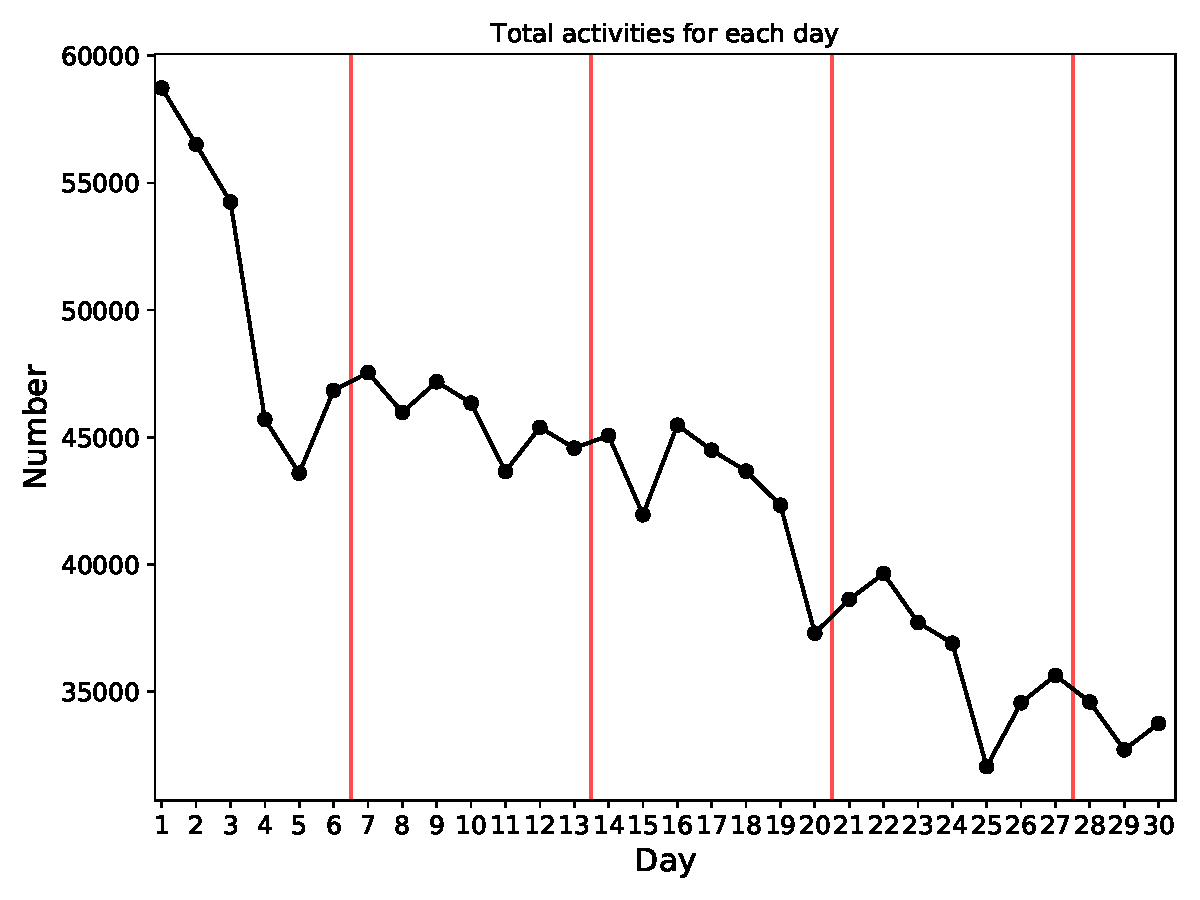
\includegraphics[width=.45\linewidth]{images/Activity/total_activities_each_day}
	}
	\caption{Le linee rosse verticali nel grafico di destra rappresentano l'inizio di una nuova settimana. Si può apprezzare un andamento complessivamente decrescente, soprattutto in corrispondenza del week-end e di festività.}
	\label{fig:activity_each_day}
\end{figure}
In Figura \ref{fig:activity_players} è possibile osservare la relazione tra numero di giocatori e attività eseguite. Come ci aspettavamo, l'andamento delle due curve risulta essere appaiato, e mantiene il trend decrescente individuato dai grafici in Figura \ref{fig:activity_each_day} e \ref{fig:playereachday}.
\begin{figure}
	\subfloat[Numero di giocatori che hanno effettuato almeno un'azione nel layer specificato ad un dato giorno.]{%
		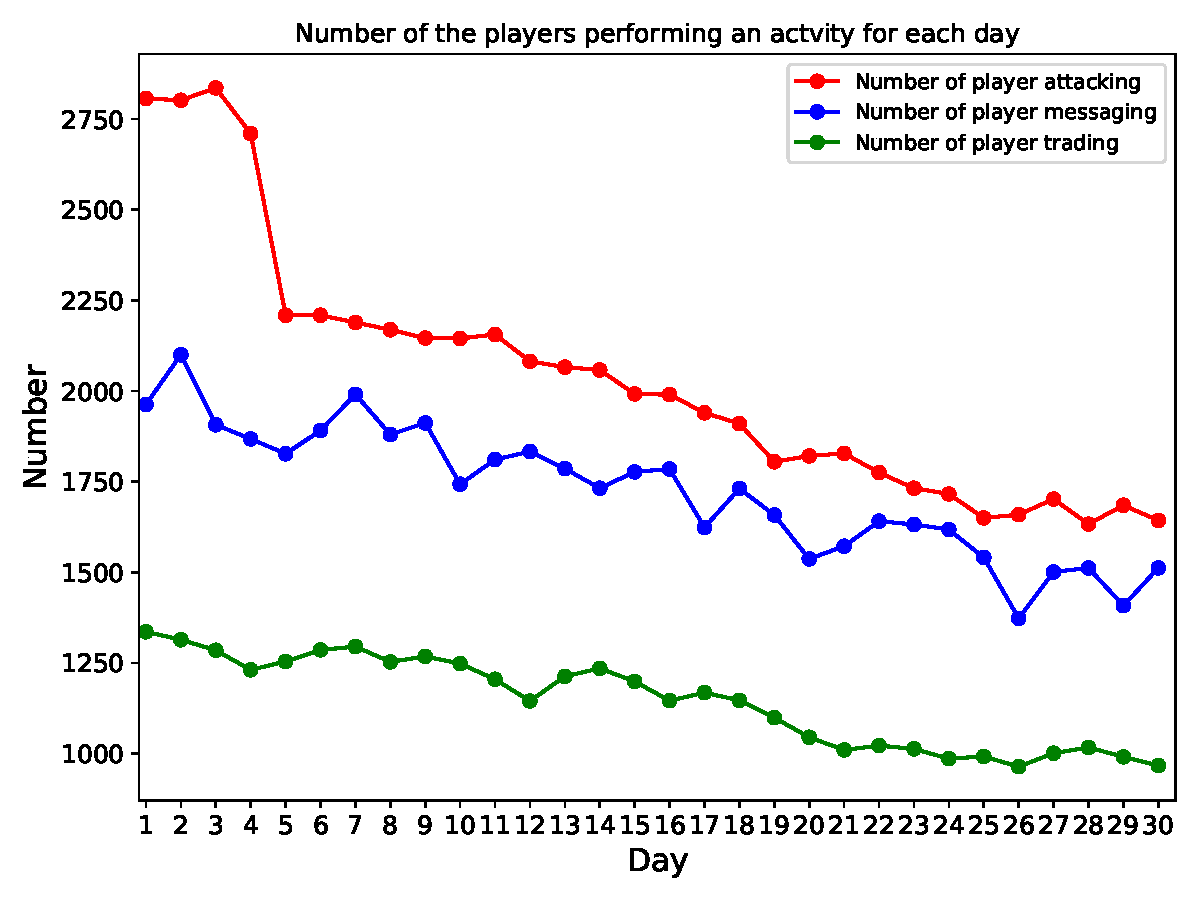
\includegraphics[width=.45\linewidth]{images/Activity/player_each_activity_each_day}
	}
	\hfill
	\subfloat[Andamento nei 30 giorni del numero di giocatori e delle attività totali.]{%
		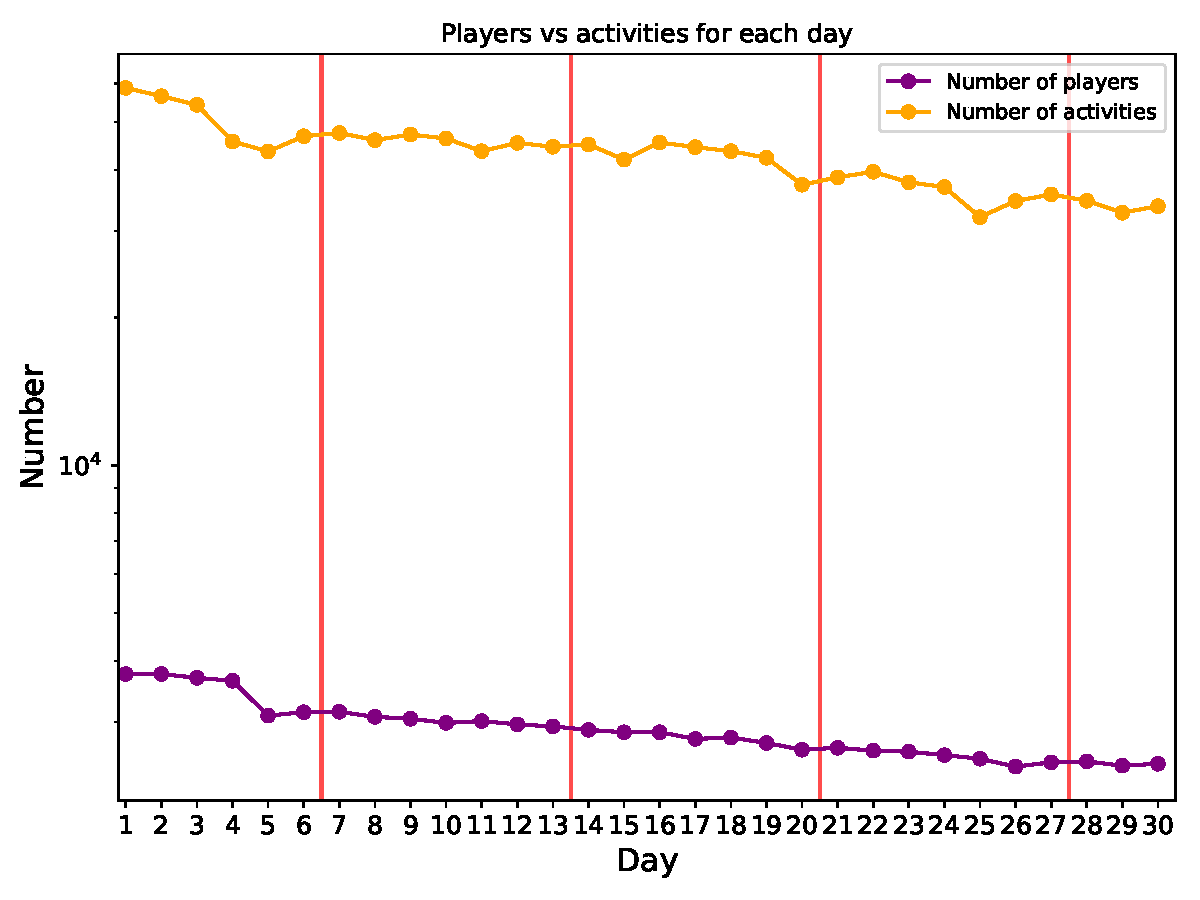
\includegraphics[width=.45\linewidth]{images/Activity/players_vs_activities_each_day}
	}
	\caption{L'andamento conferma il trend decrescente evidenziato anche in precedenza.}
	\label{fig:activity_players}
\end{figure}

In ultima battuta, abbiamo analizzato quali fossero gli orari dove si concentrasse il maggior numero di attività: in Figura \ref{fig:activity_players} sono riportati i nostri risultati. Notiamo come la maggioranza delle azioni sia eseguita tra le ore 14 e le 22, con un picco introno alle ore 18. L'andamento degli attacchi risulta essere più "liscio", probabilmente per l'elevata attività mattutina dovuta al tentativo di appropriarsi delle risorse accumulate nella notte dagli altri villaggi.\\
\begin{figure}
	\subfloat[Numero di attività per layer effettuate nei 30 giorni in una specifica fascia oraria.]{%
		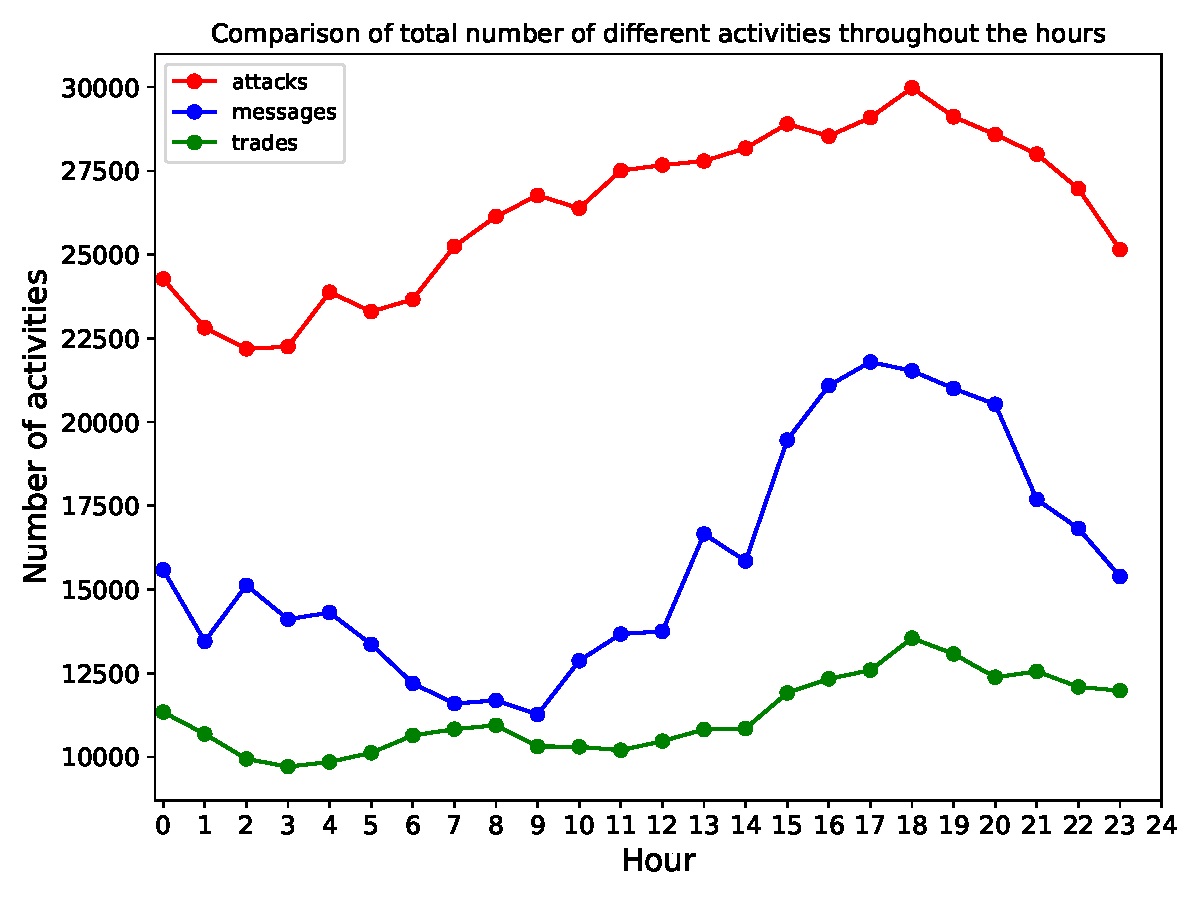
\includegraphics[width=.45\linewidth]{images/Activity/different_over_hours}
	}
	\hfill
	\subfloat[Numero di attività complessive per fascia oraria.]{%
		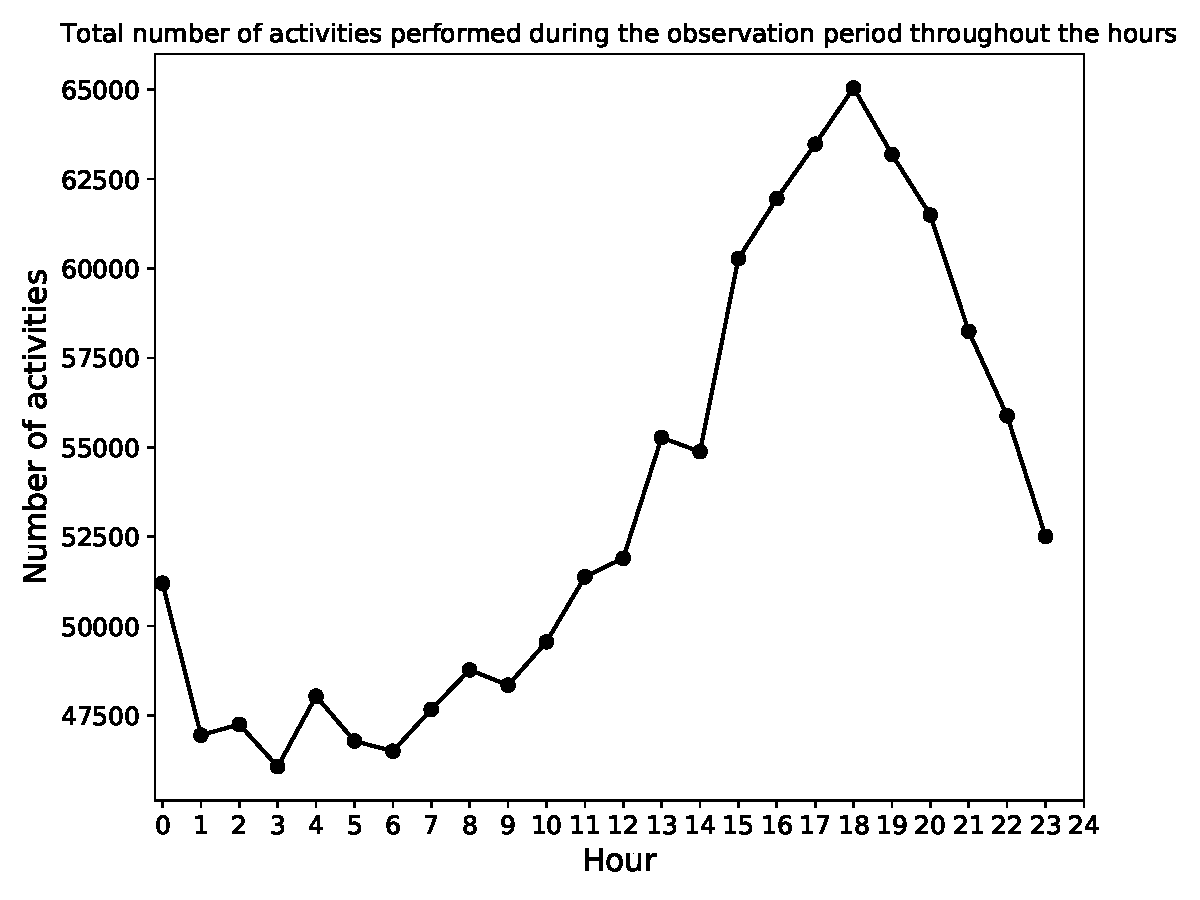
\includegraphics[width=.45\linewidth]{images/Activity/total_over_hours}
	}
	\caption{Attività sul server divisa per fascia oraria. Andamento crescente dalle ore 6 alle 18, poi decrescente fino alle 23}
	\label{fig:activity_players}
\end{figure}


\section{Ricerca di comportamenti sospetti}
Travian sostiene di aver implementato nel suo strumento di chat un metodo per impedire lo spam di messaggi verso altri utenti: se viene rilevata un grande numero di messaggi in uscita con il medesimo timestamp, il sistema blocca l'accesso del giocatore alla chat per periodi crescenti, fino al completo ban.\\
Abbiamo voluto verificare l'efficacia di questo meccanismo, cercando quei nodi con un grande numero di messaggi in uscita a cui non corrispondessero messaggi in ingresso.
Non sono stati considerati possibili spammer nodi appartenenti ad alleanze con più di 10 membri, in quanto un'attività di questo tipo potrebbe verificarsi per quelle figure che all'interno della community sono solite reclutare nuovi membri.
La nostra analisi ha confermato l'assenza di figure definibili spammer, ovvero con un rapporto messaggi inviati / messaggi ricevuti superiore a 10$\times$, e con un numero minimo di messaggi in uscita pari a 100.

\section{Ricerca di villaggi secondari}
Una pratica comune, seppur vietata dal regolamento di Travian, è quella del cosiddetto \textit{side-village} ovvero un secondo villaggio, parallelo al principale, sfruttato per la produzione di risorse che vengono poi inviate al villaggio principale sotto forma di donazione.\\
Abbiamo basato la rivelazione di questo comportamento sul rapporto tra tarde in uscita e trade in ingresso: un valore superiore a 5$\times$ ci ha fatto ritenere il villaggio come sospetto, e degno di più attente analisi da parte degli amministratori.\\
Dall'analisi sono emersi un totale di 10 villaggi sospetti, in particolare i villaggi con ID 1439, 12362, 9444, 11407, 3004, 10785, 12069, 10029, 7568, 1346.\\
Abbiamo altresì notato come a questi nodi sia associato un bassissimo grado di messaggi in entrata ed in uscita, accrescendo ulteriormente il nostro sospetto della presenza di un comportamento illecito.

\section{Studio delle community}
Il dataset presenta, in aggiunta ai file \texttt{graphml}, un file di testo contenente, giorno per giorno, tutte le alleanze registrate, con i relativi membri.\\
Al fine di effettuare analisi più approfondite su queste community, si è delineata la necessità di identificare le alleanze nel tempo e tenere traccia dei relativi membri.
La maggiore difficoltà riscontrata in questa operazione si è rivelata essere l'assegnazione di un nome univoco a queste community; i file di testo forniti contengono infatti esclusivamente gli identificatori dei nodi appartenenti ad una community, senza però stabilire a quale alleanza appartengano.
Questo è risultato essere un problema passando da un giorno all'altro, in quanto le alleanze non sono rappresentate nel medesimo ordine, e alcune si potrebbero sciogliere o creare nel frattempo.
\todo{Papetti's trick}

\subsection{Analisi della community principale}
Per determinare quale fosse l'alleanza principale contenuta nel dataset, abbiamo deciso di utilizzare come metrica la dimensione e la stabilità della community sui 30 giorni. Abbiamo così scelto l'alleanza di dimensione massima e con minore deviazione standard, che si è rivelata essere quella con identificatore 43. Riportiamo inoltre che per le 4 community più grandi la dimensione media e la relativa deviazione standard non mostrano differenze statisticamente significative.\\
Per l'analisi della community è stato analizzato il layer delle comunicazioni, in quanto abbiamo ritenuto che fosse quello maggiormente significativo per estrarre analisi interessanti dal punto di vista della rete sociale.
Sono state ripetute le misure di centralità trattate nelle Sezioni \ref{subsec:grado} e \ref{subsec:centrality}, con l'aggiunta del calcolo della closeness, ovvero una misura di quanto un nodo sia vicino al flusso informativo presente nella rete. I risultati sono riportati nelle Figure \ref{fig:comm_mean}  e \ref{fig:comm_nodes}, dove sono riportate le distruzioni delle medie delle misure e i valori per ogni nodo nei 30 giorni. Dalle distribuzioni riportare risulta evidente come vi sia una grande maggioranza di membri all'interno dell'alleanza che risultano essere poco influenti, mentre ad una parte minoritaria dei nodi sono associati valori più elevati.\\
Un'analisi approfondita mostra come valore i valori di centralità sopra la media siano associati in modo ricorrente agli stessi nodi: essi corrispondono probabilmente alle figure più rilevanti all'interno dell'alleanza, quali il leader, i suoi diretti sottoposti e figure come il reclutatore.
Emerge quindi una gestione piramidale della community, con pochi membri ai vertici ed una moltitudine di componenti poco rilevanti.
\begin{figure}
	\begin{tabular}{cc}
		\subfloat[Out degree]{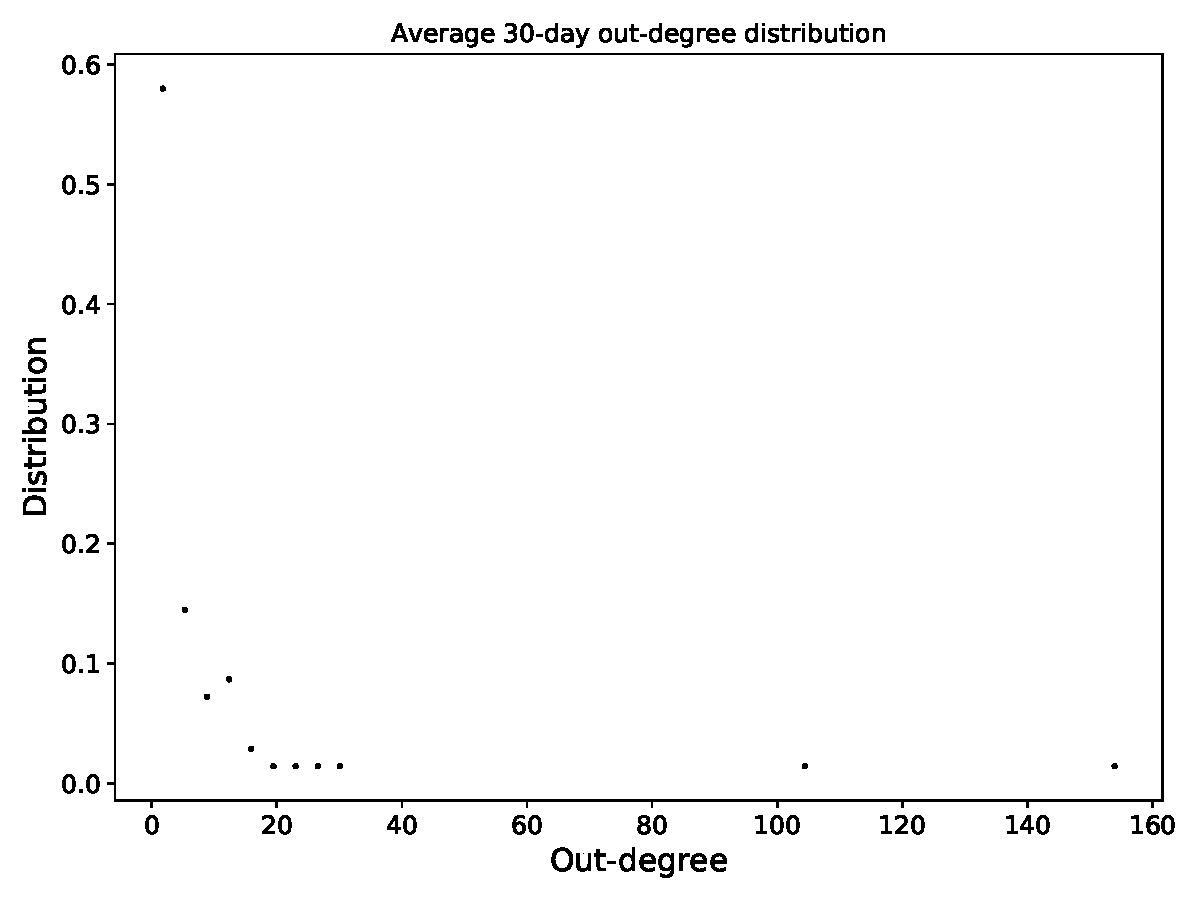
\includegraphics[width = .5\textwidth]{images/Most_important_community/distribution/out-degree_distribution}} &
		\subfloat[Betweenness]{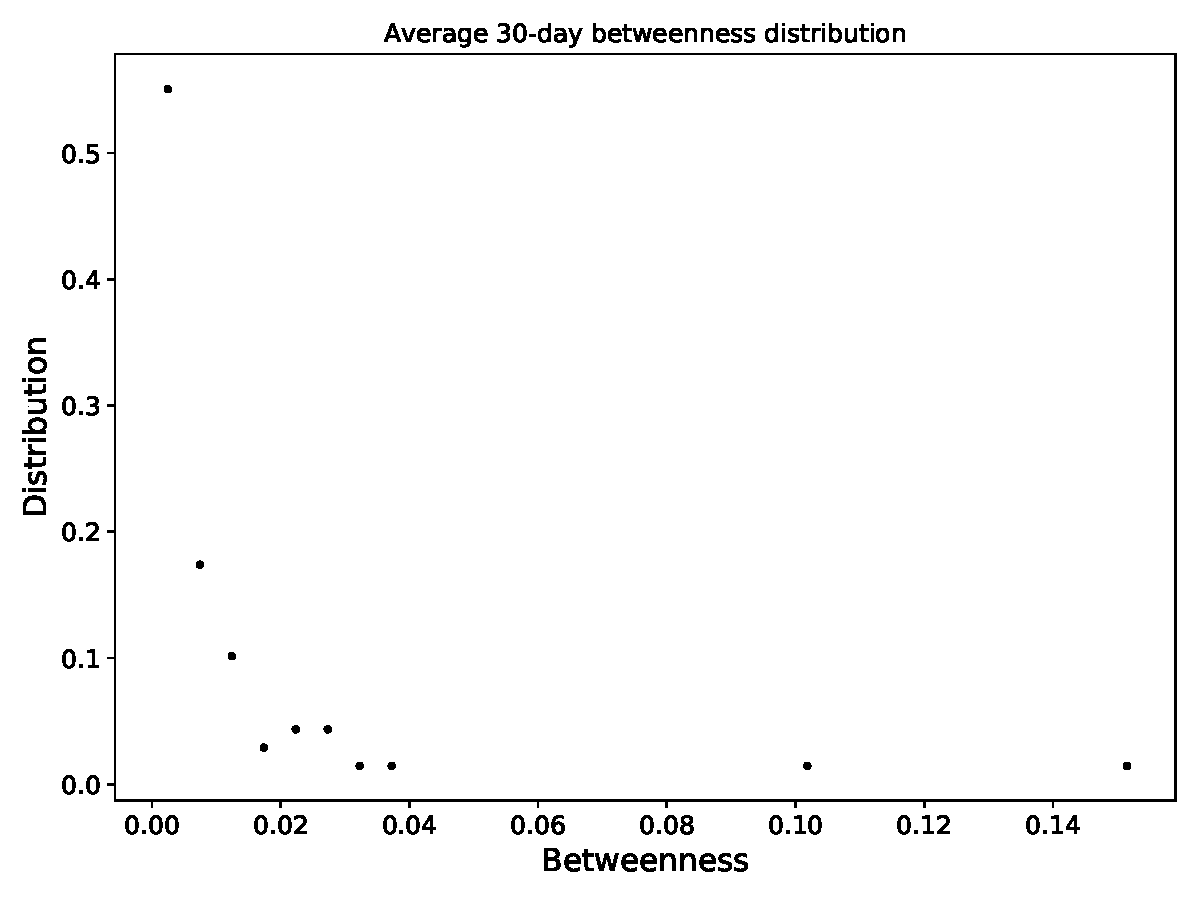
\includegraphics[width = .5\textwidth]{images/Most_important_community/distribution/betweenness_distribution}}\\
		\subfloat[Closeness]{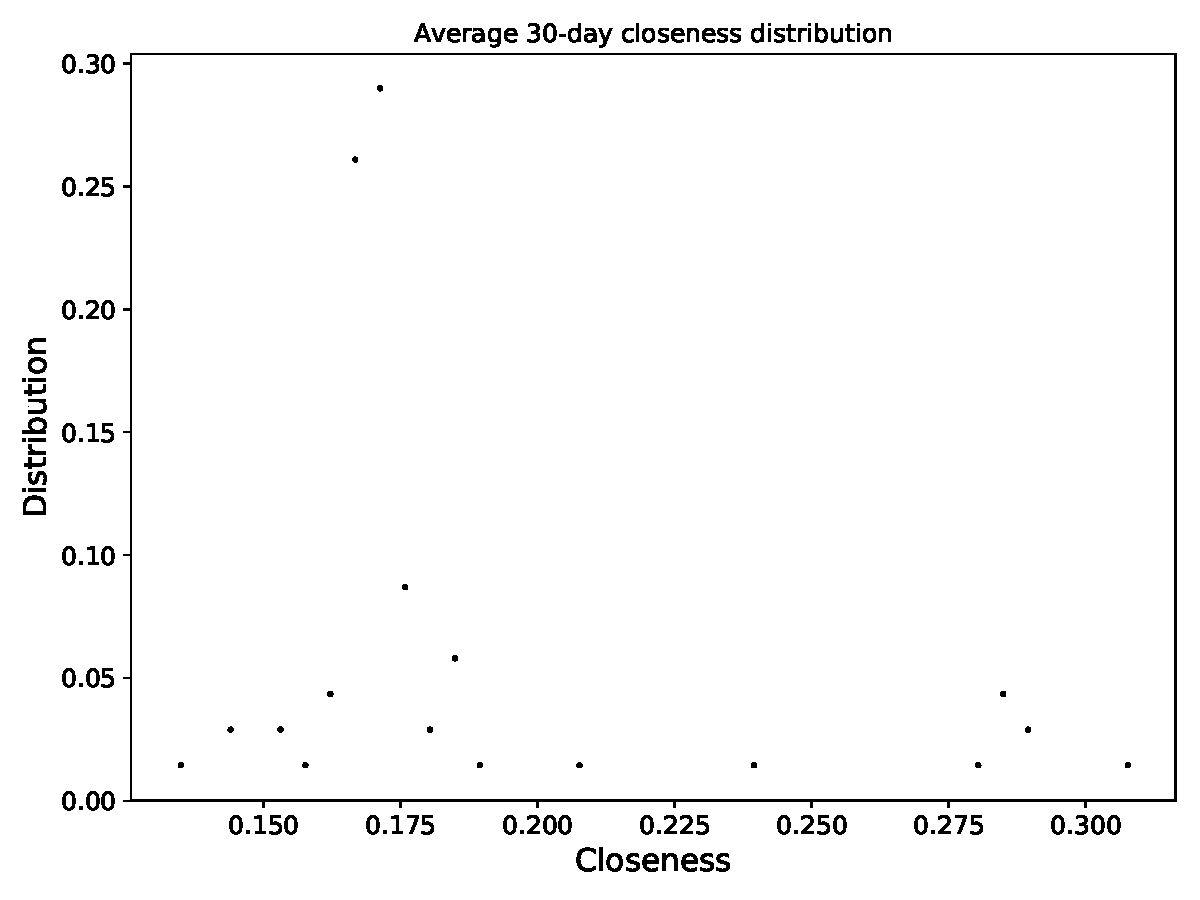
\includegraphics[width = .5\textwidth]{images/Most_important_community/distribution/closeness_distribution}} &
		\subfloat[PageRank]{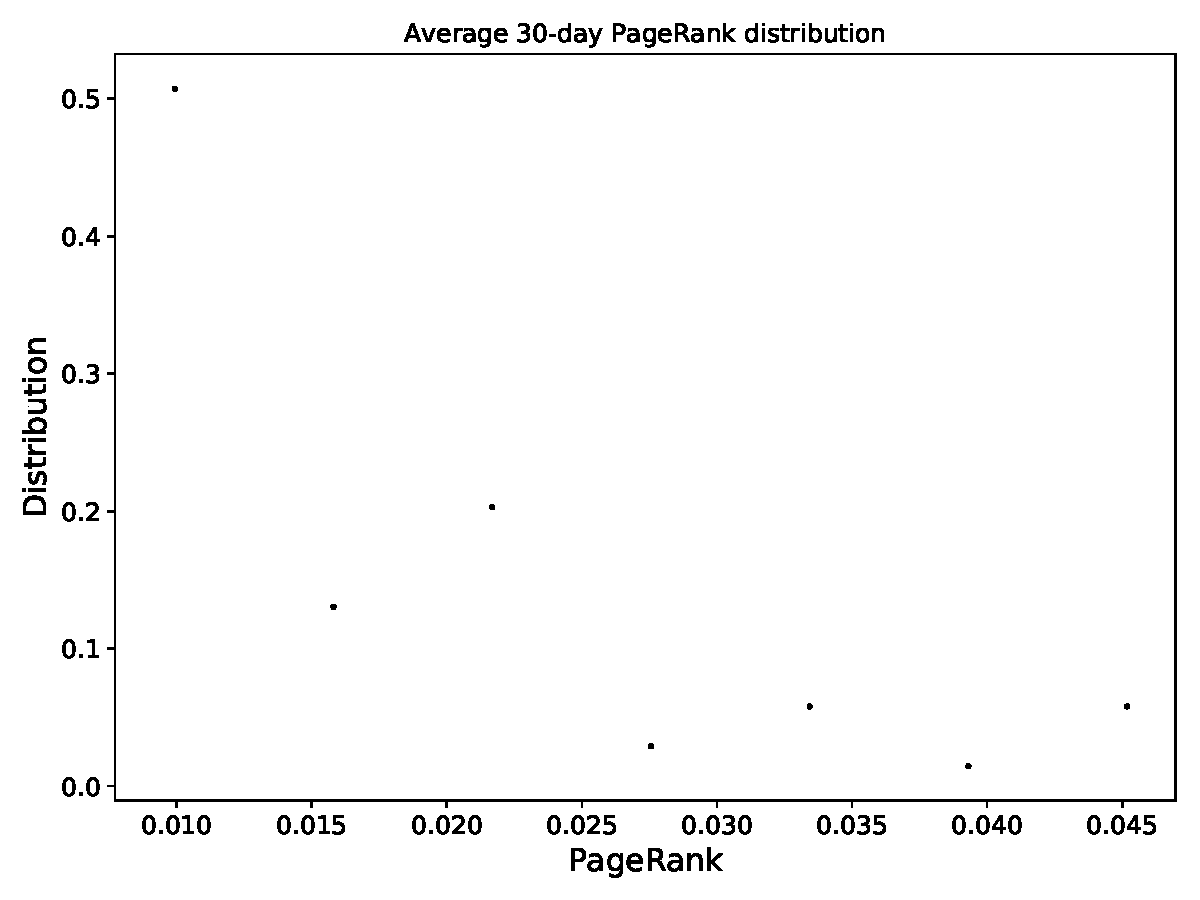
\includegraphics[width = .5\textwidth]{images/Most_important_community/distribution/pagerank_distribution}}
	\end{tabular}
	\caption{Out-degree, Betweenness, Closeness e PageRank medio sui 30 giorni.}
	\label{fig:comm_mean}
\end{figure}
\begin{figure}
	\begin{tabular}{cc}
		\subfloat[Out degree]{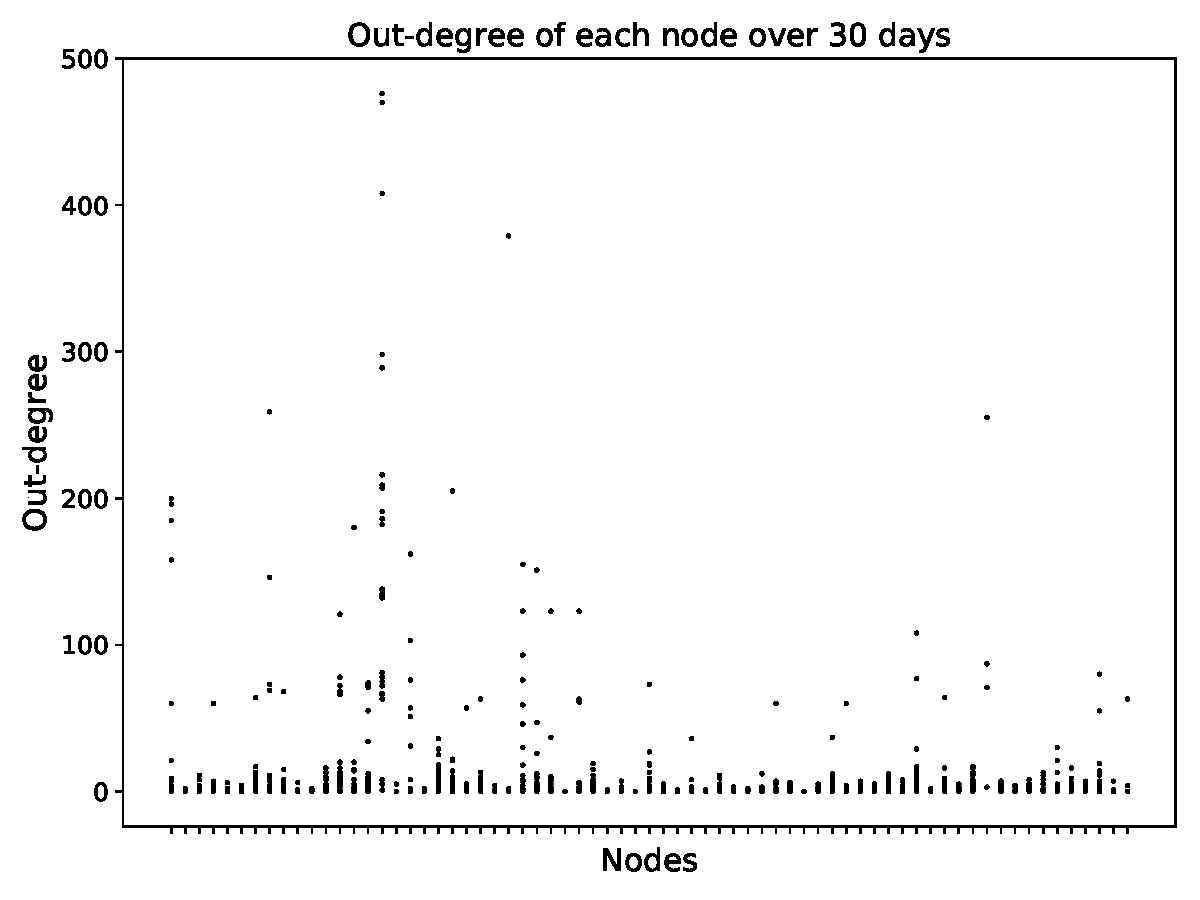
\includegraphics[width = .5\textwidth]{images/Most_important_community/each_node/out-degree_each_node}} &
		\subfloat[Betweenness]{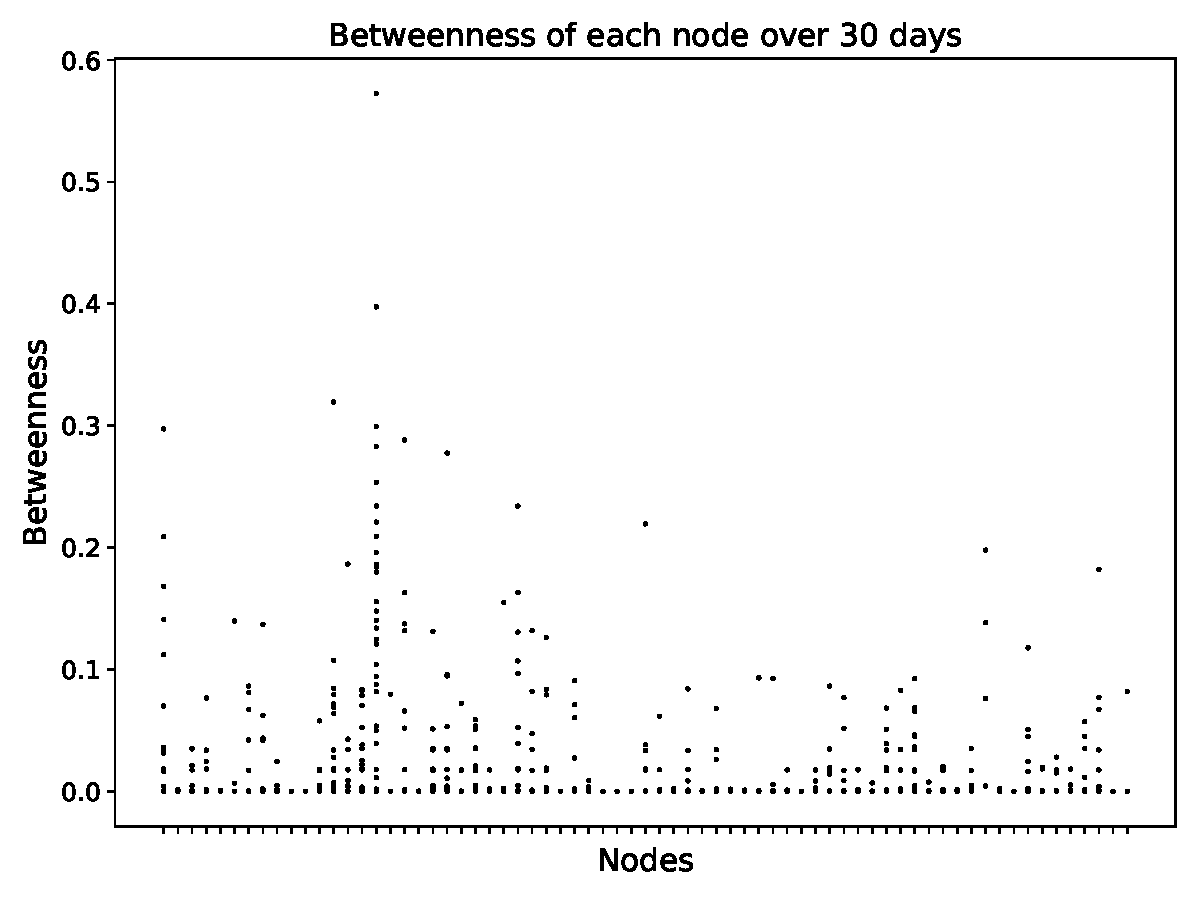
\includegraphics[width = .5\textwidth]{images/Most_important_community/each_node/betweenness_each_node}}\\
		\subfloat[Closeness]{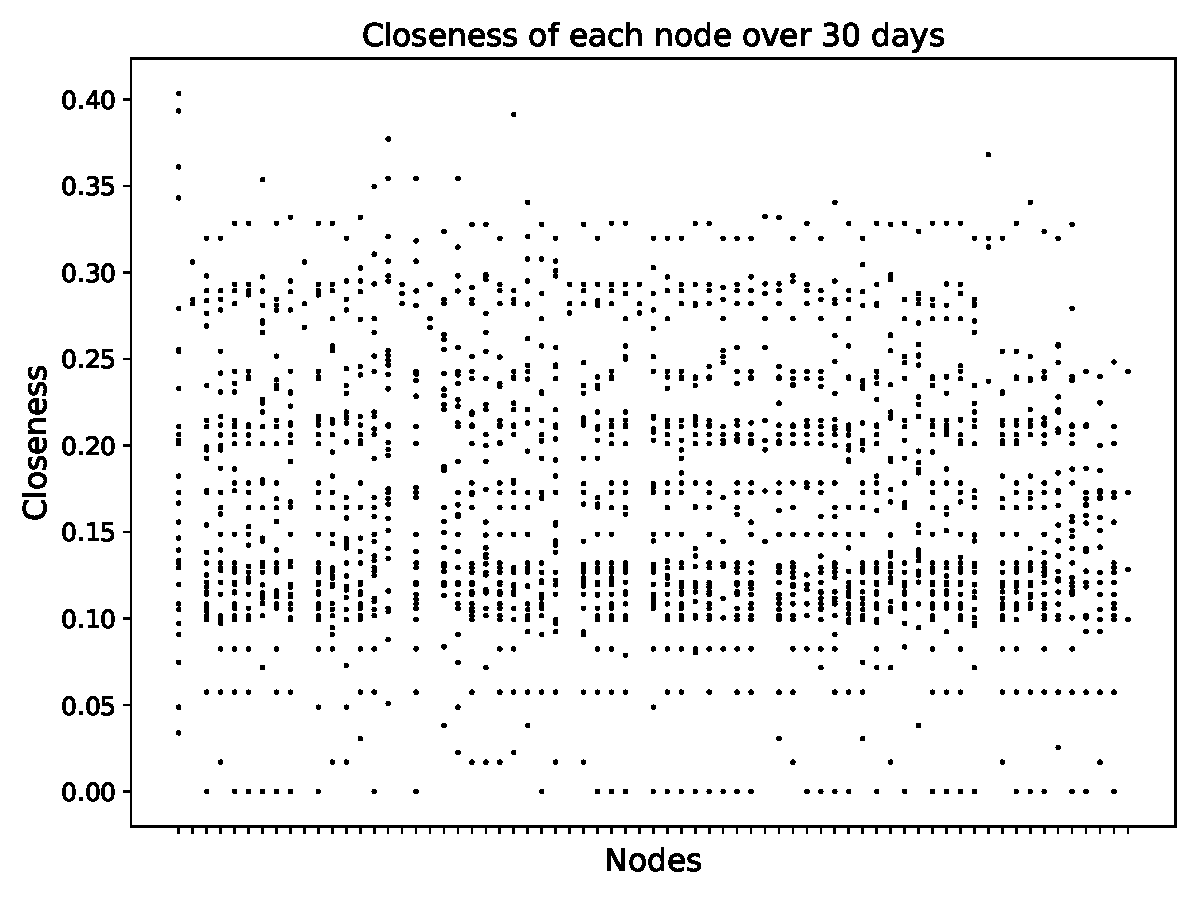
\includegraphics[width = .5\textwidth]{images/Most_important_community/each_node/closeness_each_node}} &
		\subfloat[PageRank]{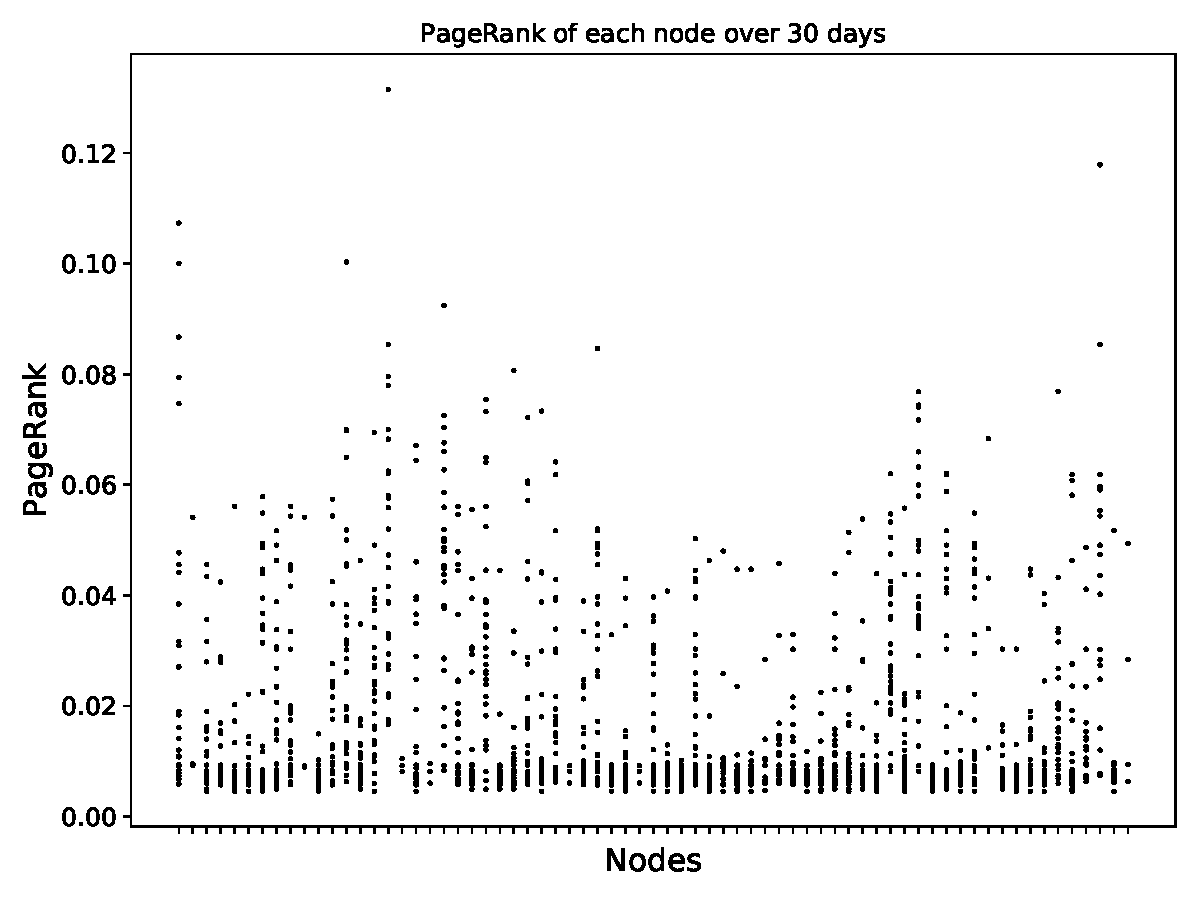
\includegraphics[width = .5\textwidth]{images/Most_important_community/each_node/pagerank_each_node}}
	\end{tabular}
	\caption{Out-degree, Betweenness, Closeness e PageRank di ogni nodo per ognuno dei 30 giorni.}
	\label{fig:comm_nodes}
\end{figure}


\subsection{Studio della densità e della reciprocità}

\subsection{Evoluzione nel tempo}

\subsection{Interazioni tra le alleanze}
\chapter{Conclusioni}
\blindtext

\todo{appendice con immagini extra}
: useremo i risultati di questa analisi come metro di paragone per i successivi studi sulle alleanze

\end{document}
